\documentclass[sigconf, nonacm]{acmart}
\settopmatter{printfolios=true}
\settopmatter{printacmref=false}
%% PACKAGES
\usepackage{graphicx}
\usepackage{hyperref}
\usepackage{cleveref}
\usepackage{subcaption}
\usepackage{natbib}
\usepackage{mathtools}
\usepackage{xcolor}

%% COLORS
\definecolor{darkgreen}{rgb}{0,0.8,0}

%% TITLES
\title{Review of ADOP: Approximate Differentiable One-Pixel Point Rendering}

%% AUTHORS
\author{Balthazar Neveu - ENS Paris-Saclay}
% \affiliation{%
%   \institution{ENS Paris-Saclay}
%   % \city{Saclay}
%   % \country{France}
% }
\email{balthazar.neveu@ens-paris-saclay.fr}


%% MAIN DOCUMENT
\begin{document}

  %% KEYWORDS
  \keywords{Neural rendering, Differentiable rendering, Point-based rendering}

  %% Teaser figure
  \begin{teaserfigure}
    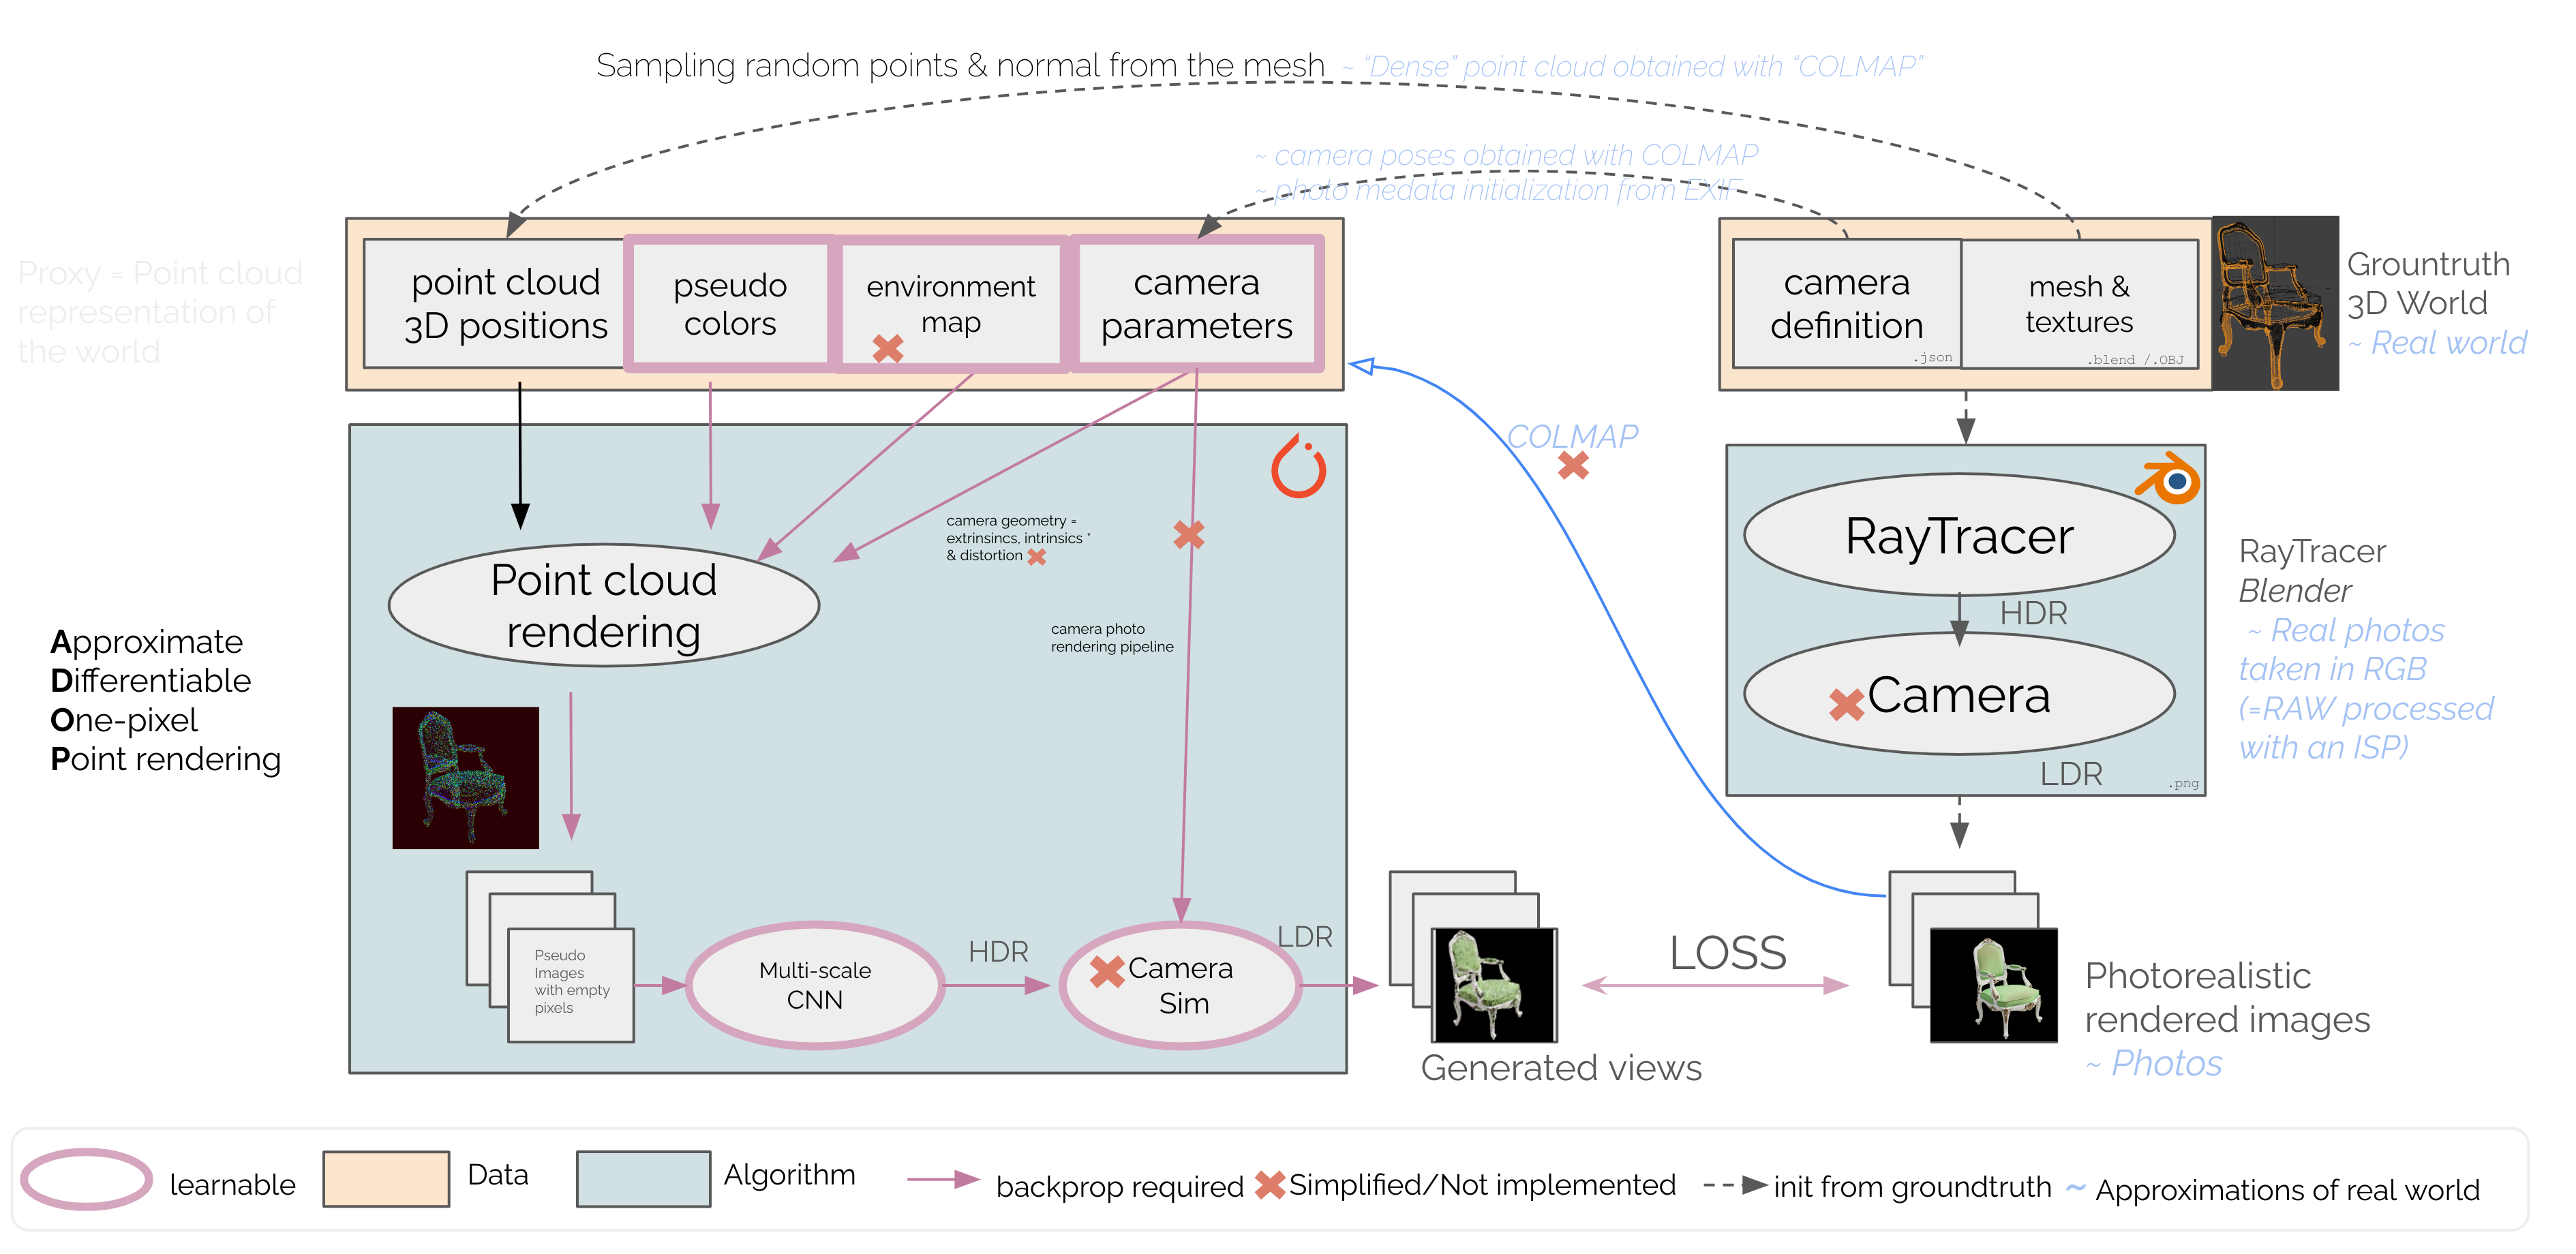
\includegraphics[width=1.\textwidth]{figures/teaser_figure_2.png}
    \centering
    \caption{Overview of our partial re-implementation to study the ADOP \cite{Aruckert2022adop} paper, in ideal conditions with calibrated scenes. \\
      \textit{Left}: Point based neural rendering reconstructs novel views from a point cloud. Original paper implementation in ADOP  works on real photos of large scale scenes. It therefore tries to model camera exposure and non linear tone mapping to adapt to each camera rendering. \\
      \textit{Right}: We mimick real world photo captures by rendering calibrated scenes and cameras (to place ourselves in the most simple conditions to review point based rendering). Point cloud is sampled randomly from the mesh with perfect normals and perfect camera poses (these would usually be estimated using COLMAP \cite{schoenberger2016sfm}). We do not let exposure vary or perform tone mapping.
    }
    \label{fig:original_pipeline}
  \end{teaserfigure}

  %% TITLE
  \maketitle




  %% CONTENT
  \section{Introduction}
\label{sec:intro}
The purpose of this report is a review of the paper ADOP: Approximate Differentiable One-Pixel Point Rendering by \citet{ruckert2022adop}.
Novel view synthesis is an intense topic of research since Neural Radiance Fields (NERF \cite{mildenhall2020nerf}) showed that a neural network could model a complex radiance field and lead to impressive novel view synthesis using volumetric rendering. NERF jointly recovers geometry and object appearace without any prior knowledge on the geometry. 
Other families of methods use a geometric "proxy" of the scene such as a point cloud \cite{Aliev2020} (or even meshes \cite{worchel2022nds}). \\
Let's put things simply: Point based rendering leads to images filled with holes and at first sight does not really look like an appropriate data structure to render continuous surfaces of objects.
We'll see how ADOP:
\begin{itemize}
    \item manages to use a point cloud structure jointly with a CNN (processing in the image space) to sample dense novel views of large real scenes.
    \item makes a special effort to try to model the camera pipeline to improve the quality of the rendered images.
    \item does not inherently have an ability to model view dependent effects such as specularities or reflections.
\end{itemize}

A re-implementation from scratch in Pytorch of some of the key elements of the paper has been made in order to understand the core aspects of the ADOP paper (which were already present in a previous paper named Neural Point Based Graphics \cite{Aliev2020}). To simplify the study, it seemed like a good idea to work on \textbf{calibrated synthetic scenes}. This way, I have been able to focus on trying to evaluate the relevance of point based rendering, see their limitations and avoid the difficulties inherent to working with real world scenes (large data and point cloud, imperfect).

\noindent Finally, my code is fully available on ~\href{https://github.com/balthazarneveu/per-pixel-point-rendering}{GitHub} and offers the possibility to generate novel views interactively.

  \section{Context}
\label{sec:Context}

\textit{ECCV 2020 : The NERF \cite{mildenhall2020nerf} paper triggers an increasing interest in the field of novel views synthesis}. Can you render novel viewpoints from a given scene using a neural network instead of running a complex ray tracing engine (in a software such as Blender)? The answer is roughly yes and... it also works on real scenes where there's no knowledge of the underlying scene. Many works try to improve the quality/speed of the rendering. We'll see how, suprisingly, point clouds can be used to render novel views of a scene.


\subsection{What is novel view synthesis?}
\label{sec:novel_view_synthesis}


\subsubsection*{Real scenes}
\label{sec:real_scenes}
Novel view synthesis is a standard computer vision task which consists in generating new viewpoints of a scene after capturing a set of images.
The concept is simple, take photographs or video of a scene by walking around it or by flying a drone.

\noindent \textbf{Camera pose estimation.} The first step is to get the camera parameters which are not necessarily known: 

\begin{itemize}
    \item pose for each capture= 6 degrees of freedom - 3 rotations and 3 translations
    \item camera intrinsics : focal length, principal point (projection of the lens optical center onto the sensor), lens distortion.
\end{itemize}

\noindent \textbf{External intialization.} Some of these variables can be pre-estimated, for instance intrinsic camera parameters can usually be pre-calibrated using the Zhang method \cite{Zhang00calib} and are assumed to be constant for the whole sequence of images \footnote{Fixed calibration is not possible when the camera has a zoom-in capabilities or auto-focus. Variable focus may also affect the focal length.}.

\noindent An IMU (inertial measurement unit) can be attached to the camera which allows later to have an estimation of the camera pose after running a sensor fusion algorithm.

\noindent But there will always be measurement errors (sensor noise, calibration error, sensor fusion errors) \footnote{Please note that efforts can be made, such as calibrating camera/IMU misalignment \cite{karpenko2011gyrostab}}.

So there's a need for an algorithm to estimate the camera poses from images, regardless of having an external pose estimation intialization.

\noindent \textbf{Structure from motion.} The traditional approach consists in using the popular COLMAP software \cite{schoenberger2016sfm} to jointly estimate camera trajectory and sparse point cloud. A side product of running this algorithm is getting a densor colored 3D point cloud of the scene (\textit{multi-view stereo being the seconde part of the COLMAP software}). 
The second step is to reconstruct a flexible representation of the scene so it can be rendered from new viewpoints. One of the technical challenge is to find the most suited data structure to represent the 3D scene subject to constraints such as: 
\begin{itemize}
    \item image / 3D structure quality: for cultural heritage or industrial monitoring applications for instance. 
    \item reconstruction time and memory consumption. Real time for AR/VR applications is a constraint. \textit{For instance, ADOP seems to take advantage of point cloud rendering hardware acceleration available in any computer using OpenGL (not necessarily with the need of a massive NVidia GPU)}. 
    \item preprocessing time: in case users want to recreate their own scenes, they may not have access to powerful GPU 
\end{itemize}

\subsubsection*{Calibrated scenes}
\label{sec:calibrated_scenes}
There's another usecase where the camera poses and scenes are perfectly known and controlled by using 3D scene synthesis. This is an easier setup to study novel view synthesis as you can truly evaluate the rendering quality of the algorithm without doubts on the quality of pose estimation (or camera photometry). This setup is sometimes refered as "calibrated scenes". One could say that representing scenes with sophisticated neural rendering is useless when you have the underlying 3D model and Blender available. Nevertheless, novel view synthesis on calibrated scenes is a good framework to test a method before deploying on real scenes.

\subsection{Representations of the scene}
\label{sec:representations}

If we solely use the colored point cloud, we'll end up with images filled with holes (when we zoom in for instance).
This is where rendering a scene start to get difficult. 
\noindent\textbf{Surface reconstruction.}It is possible to get continuous representations (without holes) by wrapping a surface around the point cloud of an object. For instance assuming we have pre-computed normals, a Signed Distance Function (SDF) defined from point cloud can be evaluated anywhere. The surface of the object is where the SDF is equal to zero. Evaluating IMLS (Implicit Moving Least Square \cite{kolluri2008IMLS}) on a fixed grid followed by the marching cube algorithm allows to recreate a mesh. All topologies may not be represented correctly (e.g. a hole in the cheese may end up being filled).


\begin{figure}[htbp]
    \centering
    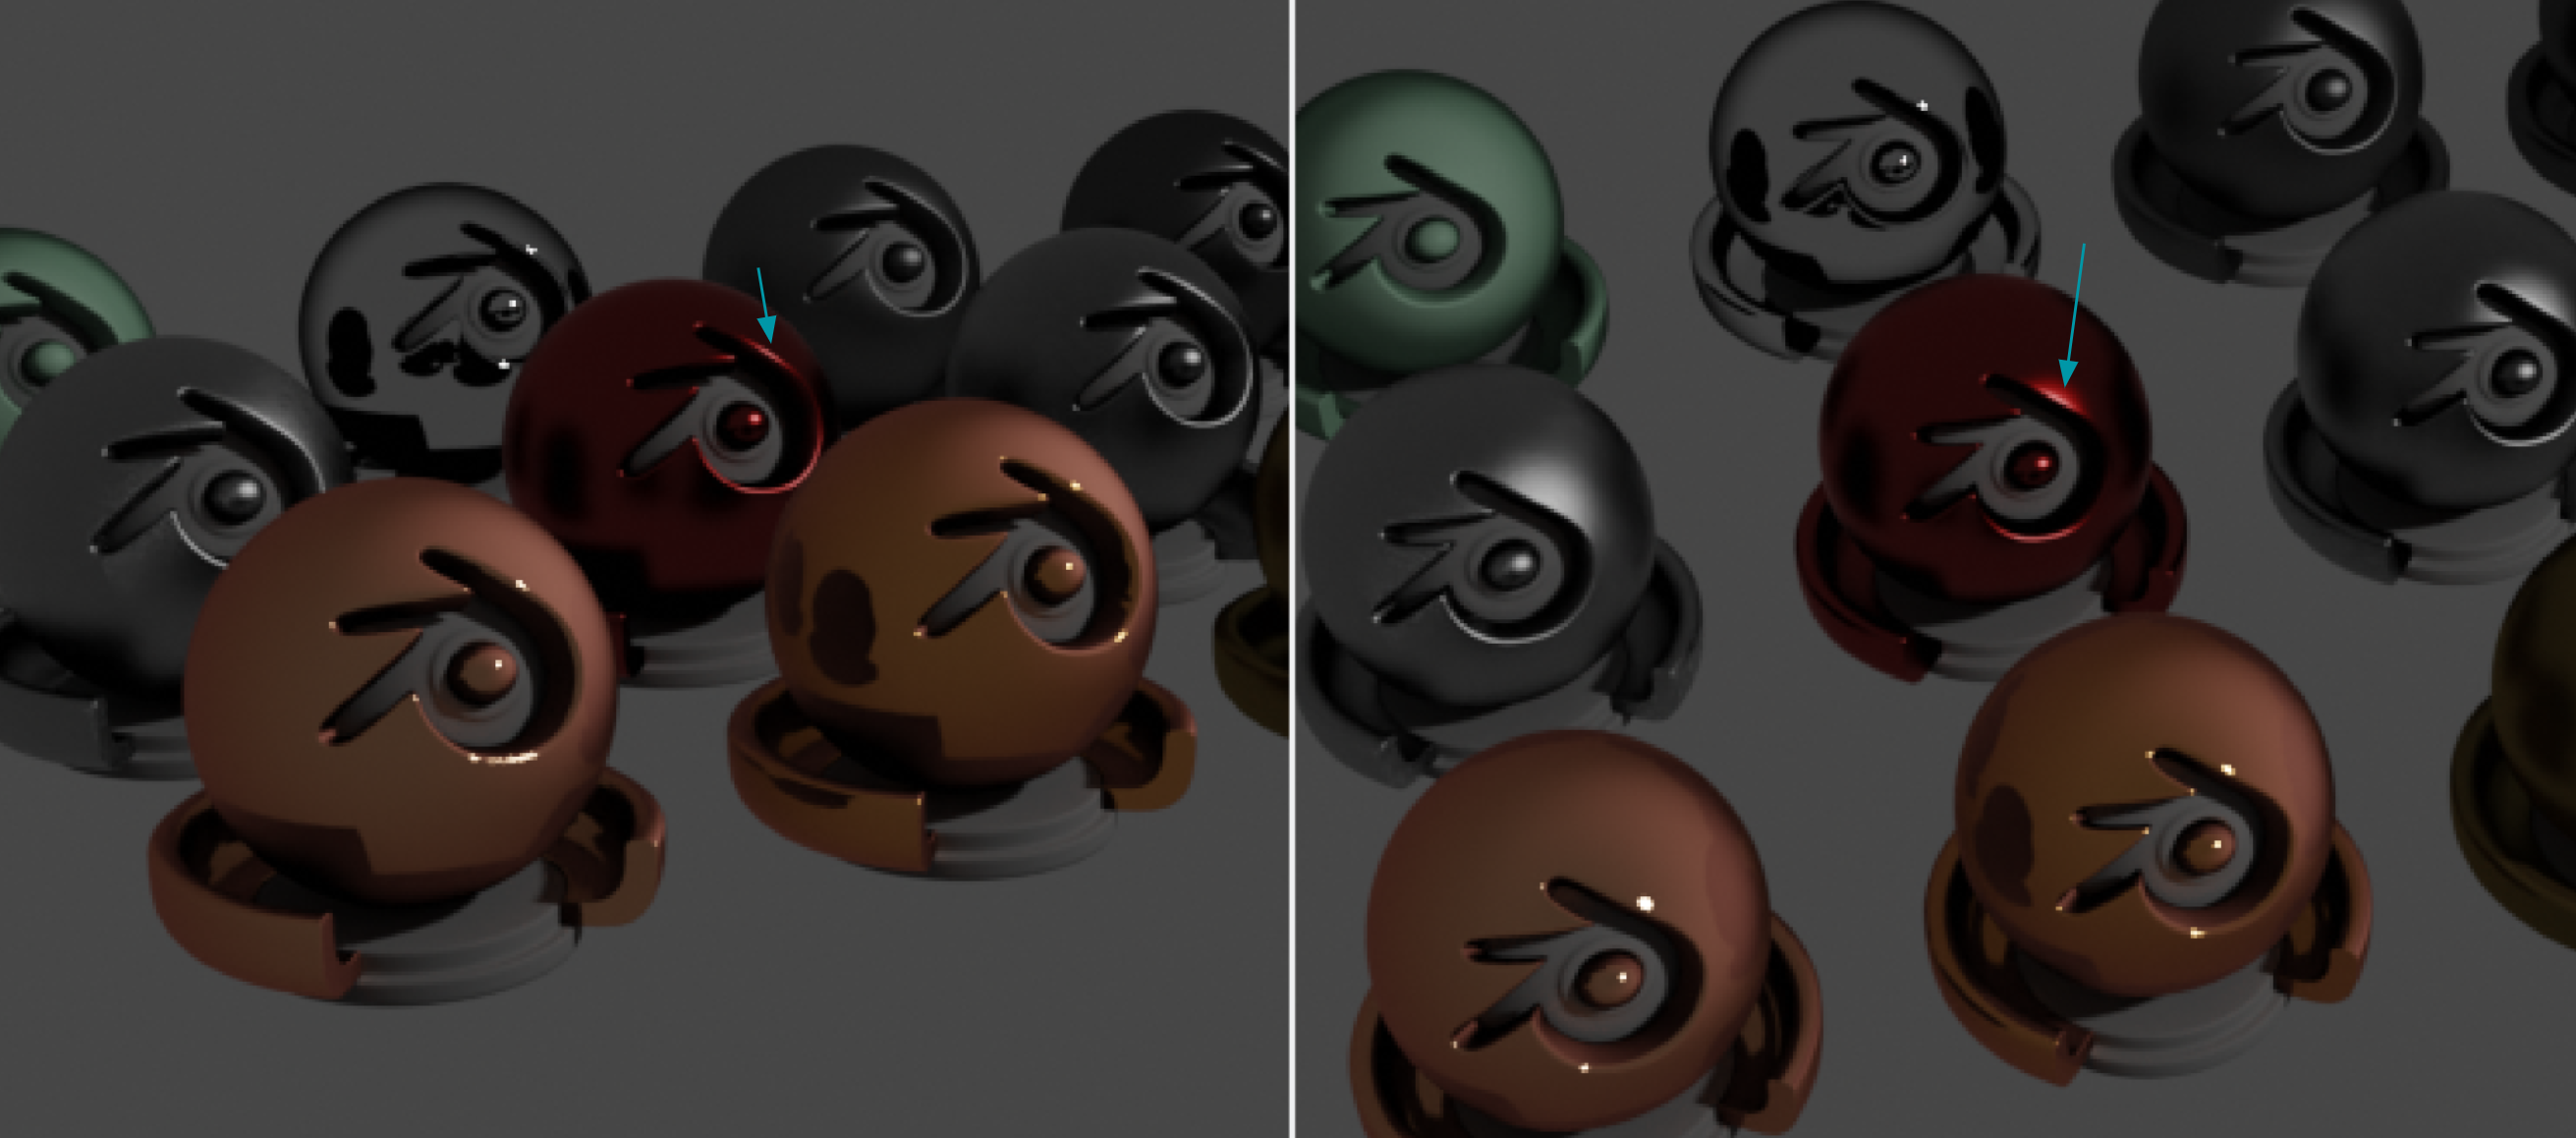
\includegraphics[width=0.5\textwidth]{figures/material_appearance_commented.png}
    \caption{Colors change with camera orientation, specular materials reflect the light and amplify this effect, the extreme use-case being mirrors.}
    \label{fig:material_changes}
\end{figure}

\noindent\textbf{Meshes.} Creating a mesh from the point cloud will lead to a nice geometric representation which can be rendered using classic rasterization techniques. But shading these triangles is still needed. If all materials are perfect diffusers, applying the textures extracted from the photos to the triangles shall be enough. Unfortunately, this will not work for specular materials as illustrated in figure \ref{fig:material_changes}. Neural deferred shading has been proposed \cite{worchel2022nds} to jointly fit a mesh while optimizing a pixel shader (mimicked by a neural network) of a classic mesh rendering pipeline (geometry processing $\rightarrow$ rasterization $\rightarrow$ \textit{(neural)} shader). Please note that the shading is baked into the scene representation and cannot be changed afterwards (for instance, lighting or materials cannot be changed).
\noindent\textbf{Neural radiance fields.} NERF \cite{mildenhall2020nerf} represents the scene colors RGB and density as a function of the 3D position and viewing angle. By shooting rays at the scene, one can integrate the estimated colors to render the final color in the image (density=0 means that the space is empty). A MLP (Multi Layer Perceptron) can approximate basically any function as long as it has enough neurons... here the MLP is used to represent the radiance field. Having the dependance on the viewing angle allows to model complex materials and lighting effects. Main drawback is that NERF are computationally expensive as they require evaluating a MLP all along the rays for each pixel...
\noindent\textbf{Point clouds.} Although point clouds are not continuous, they are a good representation of the scene and kind of easy to manipulate. The introduction of an additional inpainting method (e.g. neural rendering component) in the image space allows to overcome the limitations of the sparseness. These will be discussed in more details the next section on neural point based graphics \ref{subsec:npbg}.



\section{Methodology of the Original Paper}
\label{sec:methodology_paper}

\subsection{Paper overview}
\label{subsec:paper_overview}
ADOP \cite{ruckert2022adop} is a novel view synthesis method based on point cloud representation. 

\noindent\textbf{Geometry.} Pseudo-colors  \footnote{Pseudo-colors means a generic "feature" vector representation which can be more generic than three dimensional RGB components. A dimension 4 for instance.} assigned to each point are projected onto the camera screen at several scales. An environment map is used to model the scene background.

\noindent\textbf{Neural rendering.} The multi-scale pyramid of pseudo images will be jointly decoded and inpainted into a RGB HDR \footnote{We define HDR as high dynamic range linear RGB images - as if they'd been retrieve from a RAW 12 or 14bit sensor with sole operations black point correction, demosaicing and potentially while balance/color matrix transforms.} image at full resolution, using a U-Net architecture.

\noindent\textbf{Camera simulation.} A camera simulation module will transform the image into a LDR image \footnote{LDR stands for low dynamic range images, the ones we see on our screens after tone mapping, color adjustments like vibrancy, vigetting correction etc...}. 

% TODO: ENVIRONMENT MAP!!!!!!!!!!!!!!!!!!!!!!!!!!!!!!!!!!!!!!!!!!!!!
\noindent The whole rendering pipeline is differentiable with regard to:
\begin{itemize}
    \item the pseudo-color of each point
    \item the environment map colors.
    \item the photometry camera parameters (exposure, white balance correction, tone curve parametric vignetting...)
    \item the camera pose and intrinsics \textit{This is an approximation, but it may be useful in order to refine camera pose estimation}. 
\end{itemize}

Using several photos of the scene for supervision, all parameters (network weights, pseudo-colors, environment map and camera photo pipeline) are optimized to minimize a loss function (MSE $\mathcal{L}^{2}$ or perceptual loss\footnote{Perceptual loss \cite{johnson2016perceptual} optimizes the distance between two images in a latent space rather than in the RGB colors space. We usually minimize the $\mathcal{L}^{2}$ distance between the feature maps in the middle of a frozen VGG network}) between predicted LDR rendered images and the real ones. 



\subsection{Neural Point Based Graphics}
\label{subsec:npbg}
NPBG \cite{Aliev2020} (Neural Point-Based Graphics) introduced several important concepts which will be discussed in the next section.
The idea of filling the holes between projected points by using multi-scale convolutional neural networks.  

\subsection{Point based Rendering}
\label{subsec:Point based Rendering}
One of the major advantage of point based methods is that this technology is backed by years of prior industy work. Rendering point clouds can be hardware accelerated and is available to the mainstream public on basically any computer (without NVidia GPU). Libraries such as OpenGL offer the option to render points \texttt{GL\_Points} (and even specify the size of the splat \texttt{glPointSize(1);})... Point clouds can even be rendered in a web browser as shown in figure \ref{fig:potree}.

% https://github.com/rougier/python-opengl/blob/master/07-points.rst
% https://glumpy.github.io/

\begin{figure}[htbp]
    \centering
    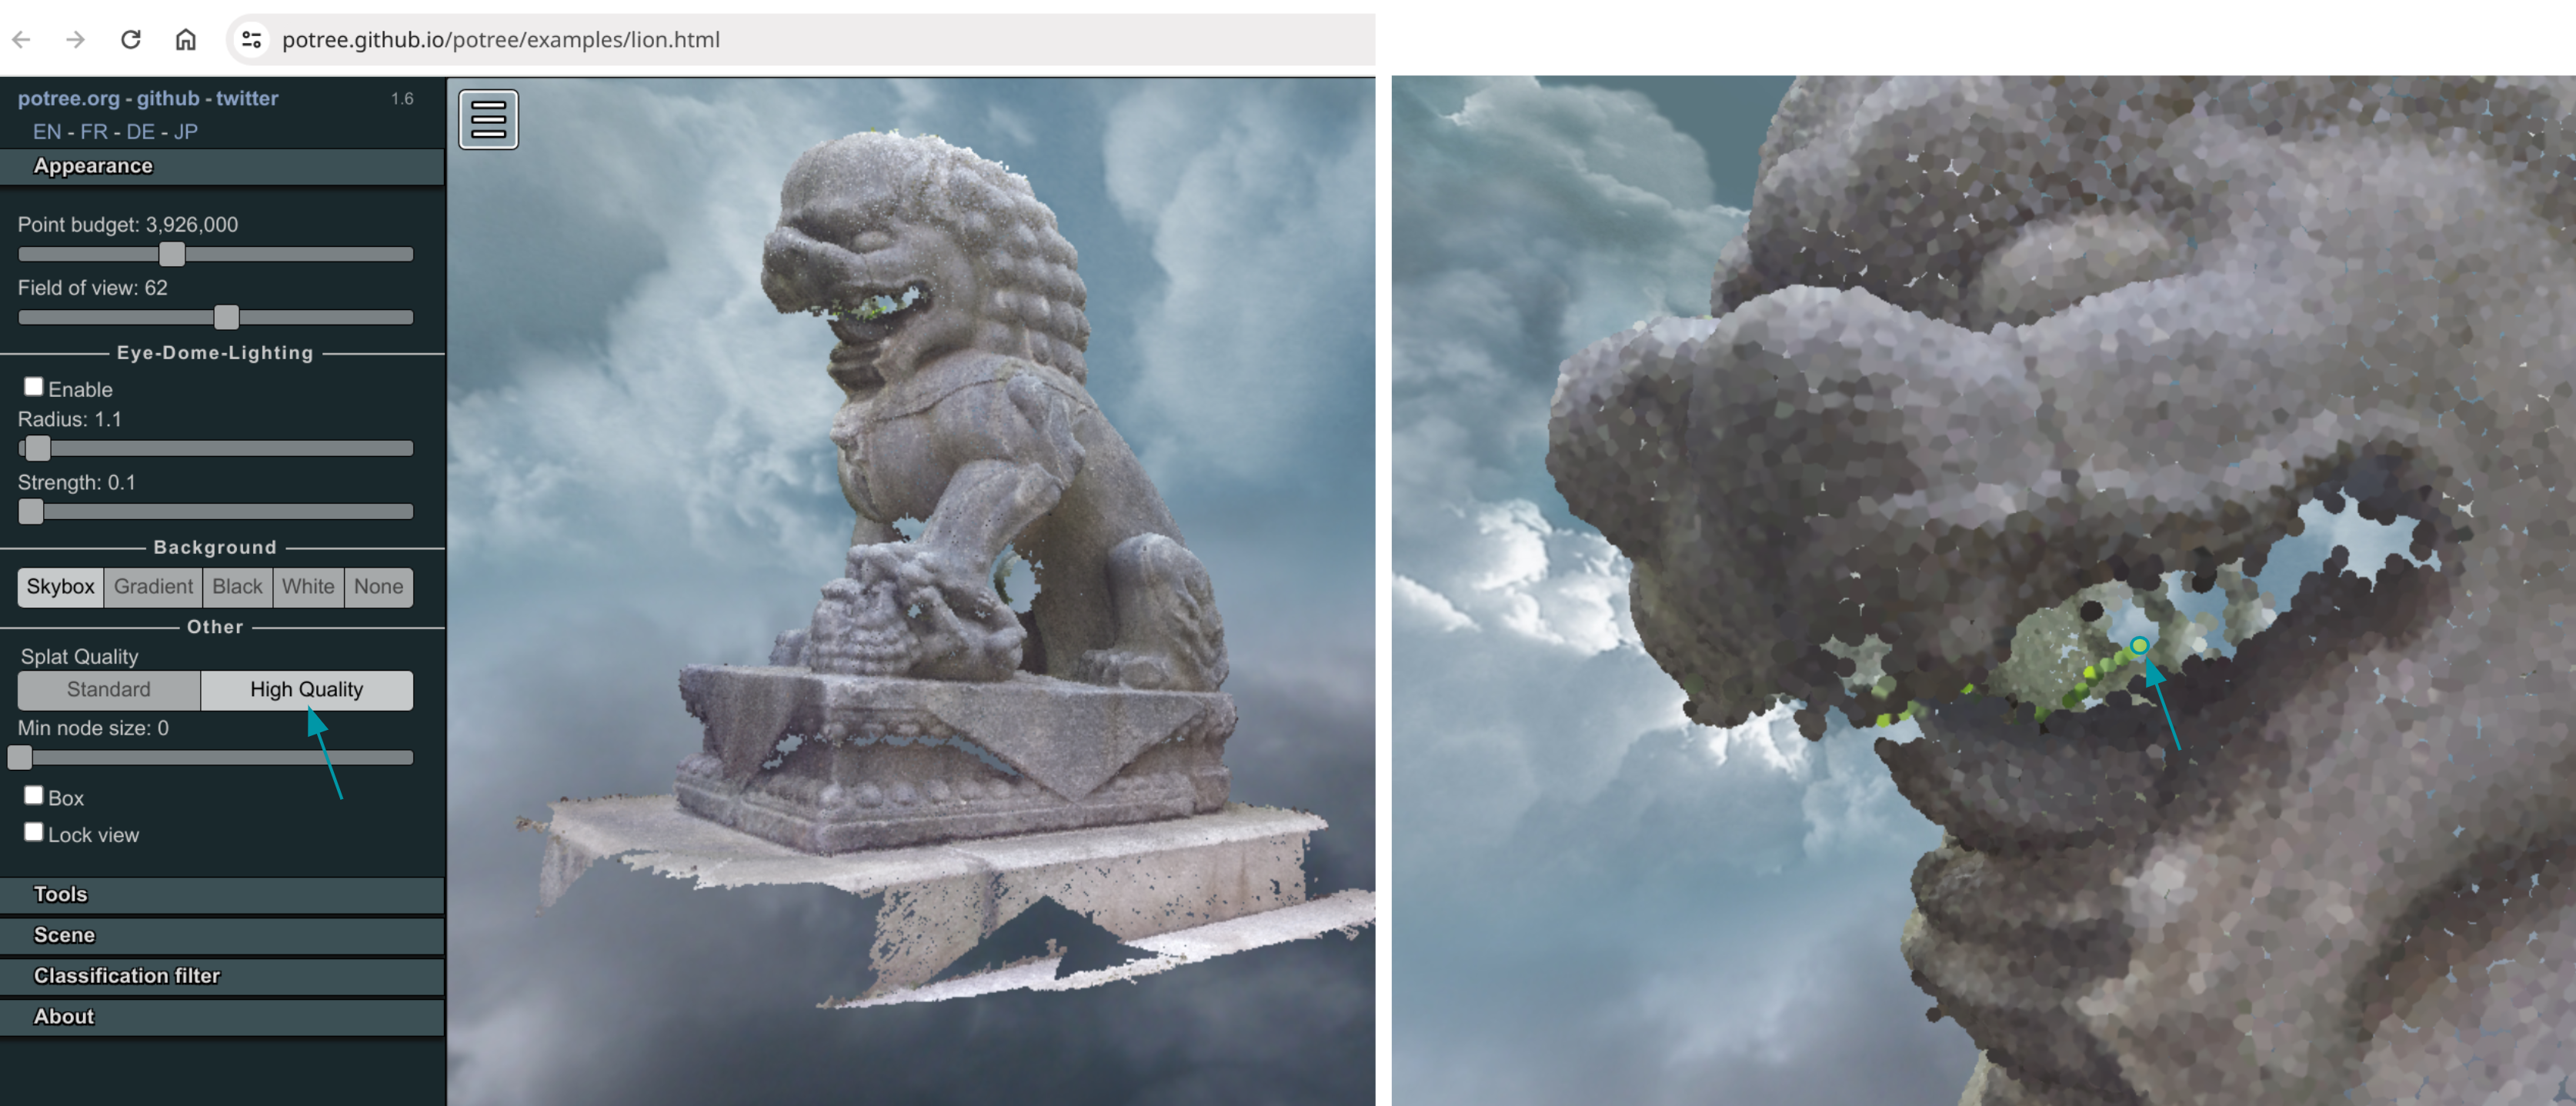
\includegraphics[width=0.5\textwidth]{figures/potree_rendering_and_splat.png}
    \caption{Potree \cite{potree} allows point cloud rendering in the browser, points being rendered as tiny circles splatted on the screen.}
    \label{fig:potree}
\end{figure}



\subsection{Novel view}
\label{subsec:Projecting points}



\noindent\textbf{Implementation.} The authors used lib Torch to compile the code. 




\subsection{Limitations}
\label{subsec:Projecting points}

  \section{Reimplementation Strategy}
\label{sec:remplementation}

The main purpose of my implementation work was to be able to code by myself some of the core ideas of the ADOP differentiable point based neural renderer.
I decided to code everything from scratch knowing since the start that I would at no point be able to fully reproduce the results from the authors but I learnt a large amount of things by doing so.
\begin{itemize}
    \item I used BlenderProc \cite{Denninger2023} to script and generate multiple synthetic scenes from the samples used in the NerF paper. All camera positions are known and share the same referential as my pytorch point renderer.
    \item A perfect point cloud is sampled at random from the mesh (through the .obj file).
    \item A few pytorch based function allows to project the points onto the image plane and include soft depth test and normal culling.
    \item A CNN is trained to predict the right dense color of the points in the image space.
\end{itemize}

Each element has been carefully tested by mostly visual tests.
Below is the list of all simplifications that have been made compared to the original ADOP paper.
\begin{itemize}
    \item We assume linear RGB cameras without tone mappings.
    \item We discard environment map (e.g. our background is black).
    \item We generate photorealistic renders of synthetic meshes instead of using real photos. 
    \item Camera poses are perfectly known.
    \item We do not refine the camera poses (no need to be approximately differentiable with regard to camera geometry parameters).
    \item Using meshes allows us sampling point clouds with normals without estimation errors such as the one we'd face with COLMAP.
    \item We can easily control the number of points to be able to test on a limited capacity GPU with only 4Gb of RAM.
\end{itemize}

\begin{figure}[H]
    \centering
    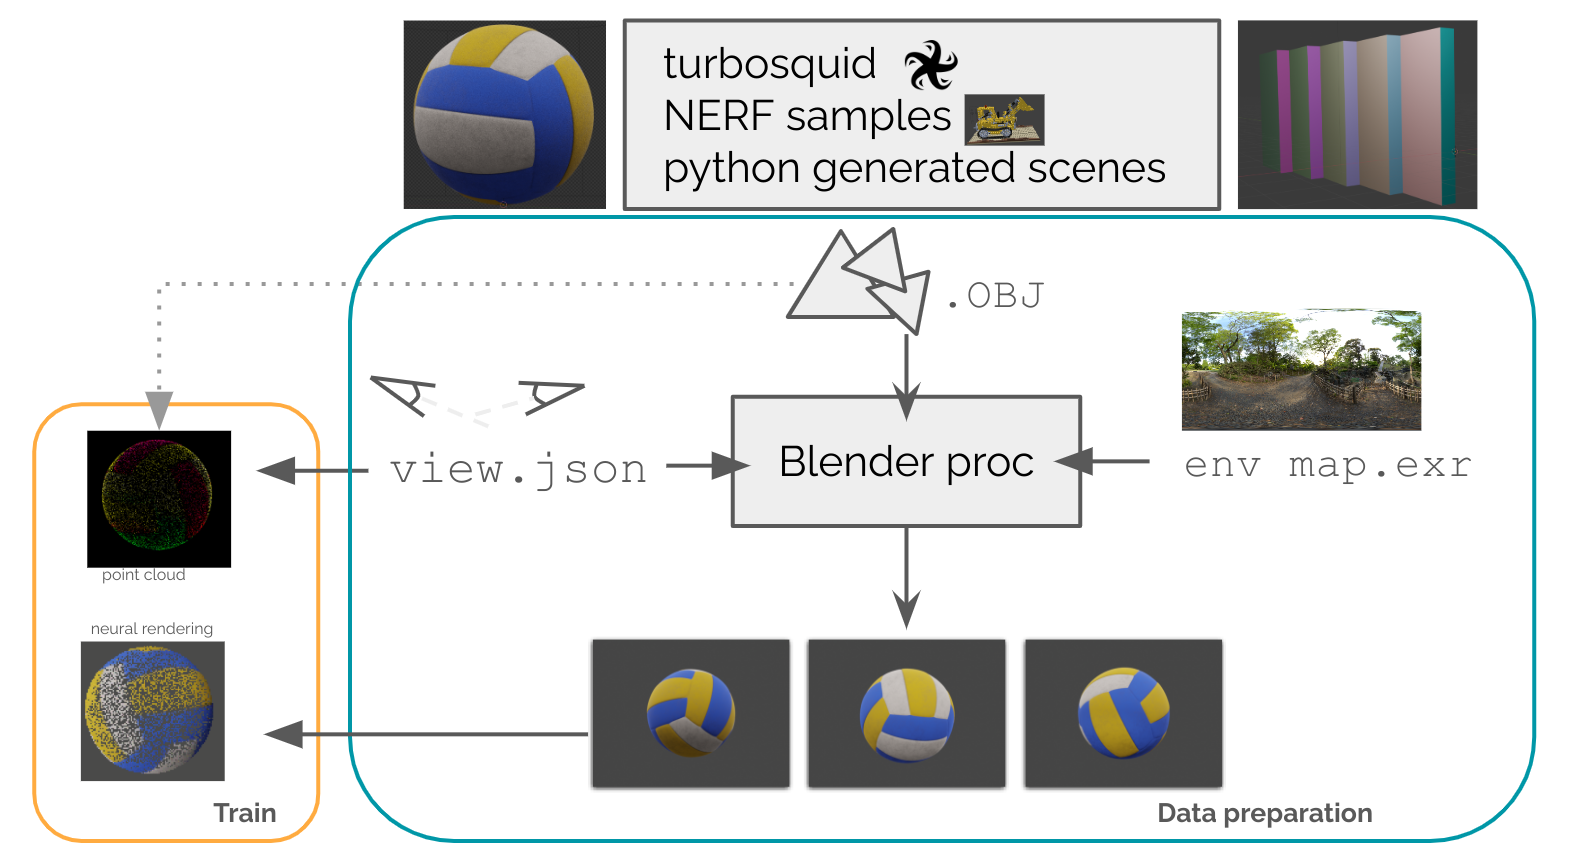
\includegraphics[width=0.5\textwidth]{figures/data_prep_and_training.png}
    \caption{Workflow: \href{https://github.com/balthazarneveu/per-pixel-point-rendering/blob/main/studies/photorealistic\_rendering.py}{\texttt{photorealistic\_rendering.py}} allows preparing camera multiviews positions saved as \texttt{.json} files in order to render photorealistic views of a \texttt{.blend} or  \texttt{.obj} files which come from internet resources or test scenes generated in python.
    The .obj and view .json files tie together the BlenderProc rendering and my Pytorch point rendering implementation: The point cloud is sampled from the mesh and the camera poses are known. A neural network is trained using \href{https://github.com/balthazarneveu/per-pixel-point-rendering/blob/main/scripts/optimize\_point\_based\_neural\_renderer.py}{\texttt{optimize\_point\_based\_neural\_renderer.py}} to predict colors of the points by trying to match the multiple photorealistic renderings. CNN weights, pointcloud, normals and pseudo-colors are all saved along in a \texttt{.pt} file which later allows performing live novel view synthesis \href{https://github.com/balthazarneveu/per-pixel-point-rendering/blob/main/scripts/novel\_views\_interactive.py}{\texttt{novel\_views\_interactive.py}} based on the self developped \href{https://github.com/balthazarneveu/interactive\_pipe}{interactive\_pipe} library}.
    \label{fig:data_and_train}
\end{figure}


\subsection{Generating synthetic calibrated scenes}
\label{sec:synthetic_calibrated_scenes}
In order to avoid dealing with large real scenes with millions of points and having to deal with heavy COLMAP processing, I decided to use a recent library named BlenderProc  \cite{Denninger2023} which simplifies the use of Blender as it allows running renders in the background (launched through terminal without the need of a graphical user interface).

It is first possible to generate a set of viewpoints configurations to orbit around the scene. It is also possible to generate an environment map (e.g. a skybox). We render with the background transparency option so the rendering results is a RGB PNG. 
% 1532.9s for 60 views of the \texttt{material balls}.
% 753.869 ficus

% Rendering is peformed using GPU and requires 25 seconds per view with a resolution 640x480 for the \texttt{material balls}. scene on a laptop Nvidia T500.
% 27 minutes are needed to generate 64 viewpoints
\begin{figure}[H]
    \centering
    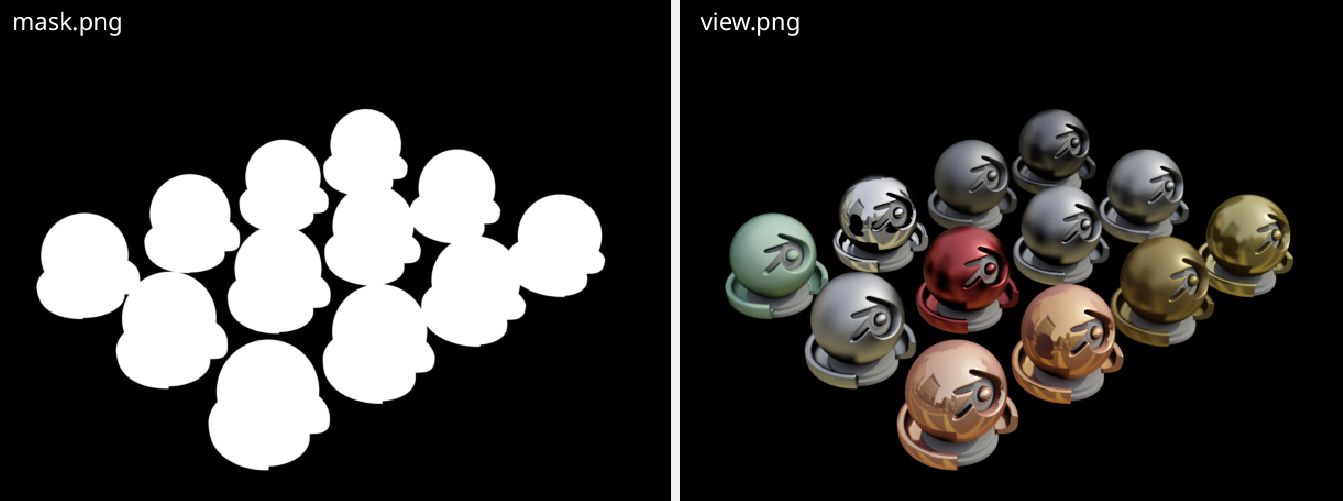
\includegraphics[width=0.5\textwidth]{figures/blenderproc_renders.png}
    \caption{Mask and RGB render BlenderProc renders with an environment map.}
    \label{fig:blenderproc_renders}
\end{figure}

\begin{figure}[H]
    \centering
    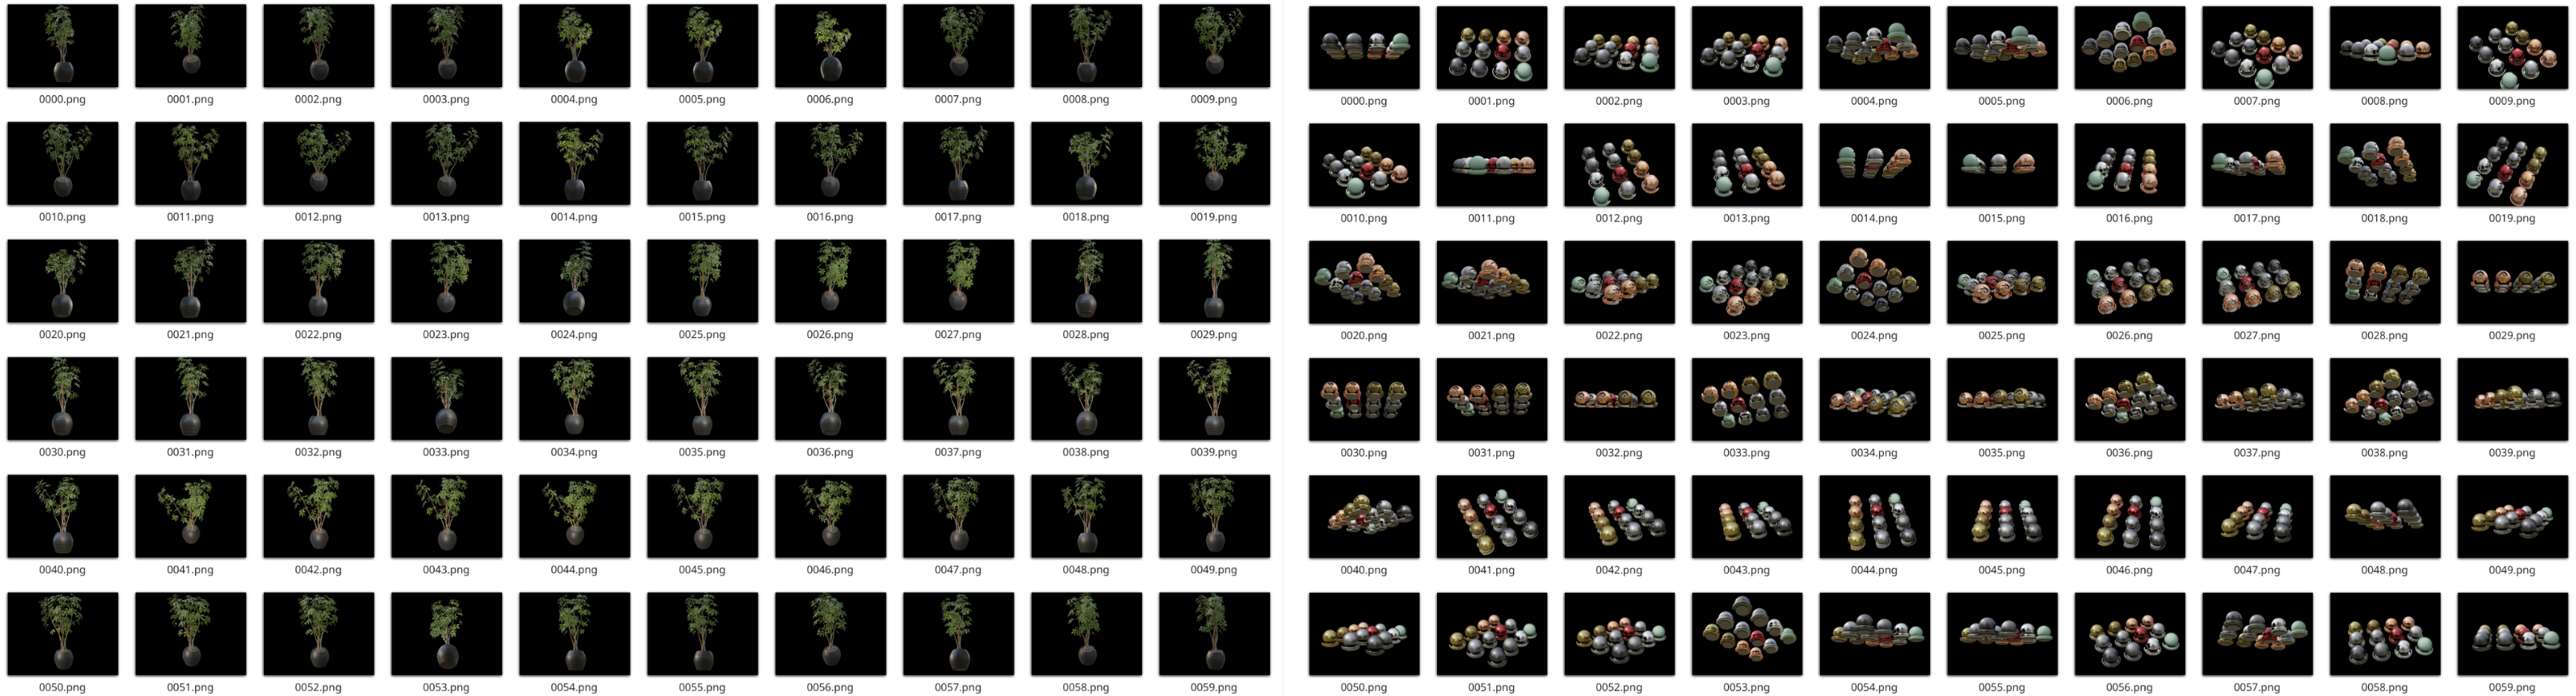
\includegraphics[width=0.5\textwidth]{figures/ficus_and_matballs.png}
    \caption{60 views of resolution 640x480 of the \texttt{Ficus} scene rendered in 12 minutes On the right, \texttt{material balls} scene rendered in a total of 25 minutes on a laptop equipped with a Nvidia T500.}
    \label{fig:multiview}
\end{figure}

Using the environment map as a background has been disabled in BlenderProc as it allows to simplify and remove one of the extra components of the ADOP paper (e.g. it allows rendering the point cloud without using the neural environment map trick and we use black uniform color instead).

We parameterize camera orientation using 3 Euler Angles (yaw pitch roll) and 3 positions. We build the extrinsic camera matrix from the 3 angles and use a pinhole camera model to project 3D points onto the image plane as we'll see in ~\cref{sec:projecting_the_point_cloud_onto_the_image_plane}. There's a perfect equivalence between the camera parameters used in Blender and the ones used in my Pytorch renderer.

One of the difficulties of using synthetic rendering from meshes is that sometimes thin surfaces are modeled with double sided triangles. Since our rendering pipeline is using normal culling, we end up with an issue: points with normals not pointing towards the camera are not rendered. So on the ficus scene for instance, if we look "at the green leafs" from the bottom, the green leaves will become transparent so the renderer will have a hard time during reconstruction. We may therefore stick to objects with easy geometry such as the \texttt{old chair} scene. This is illustrated in \cref{fig:ficus_culling_issue}.

When working on natural scenes, the points will most probably be duplicated on both sides of the surface by COLMAP with the normals in both ways. In my case, I sampling points randomly from the mesh and I simply take the normal of the triangle to which the point belongs without considering it double sided.

I first notticed this effect on my synthetic \texttt{stair case} scene which was only made of planes and that could not be optimized in the trivial "Bypass" case.

\begin{figure*}
    \centering
    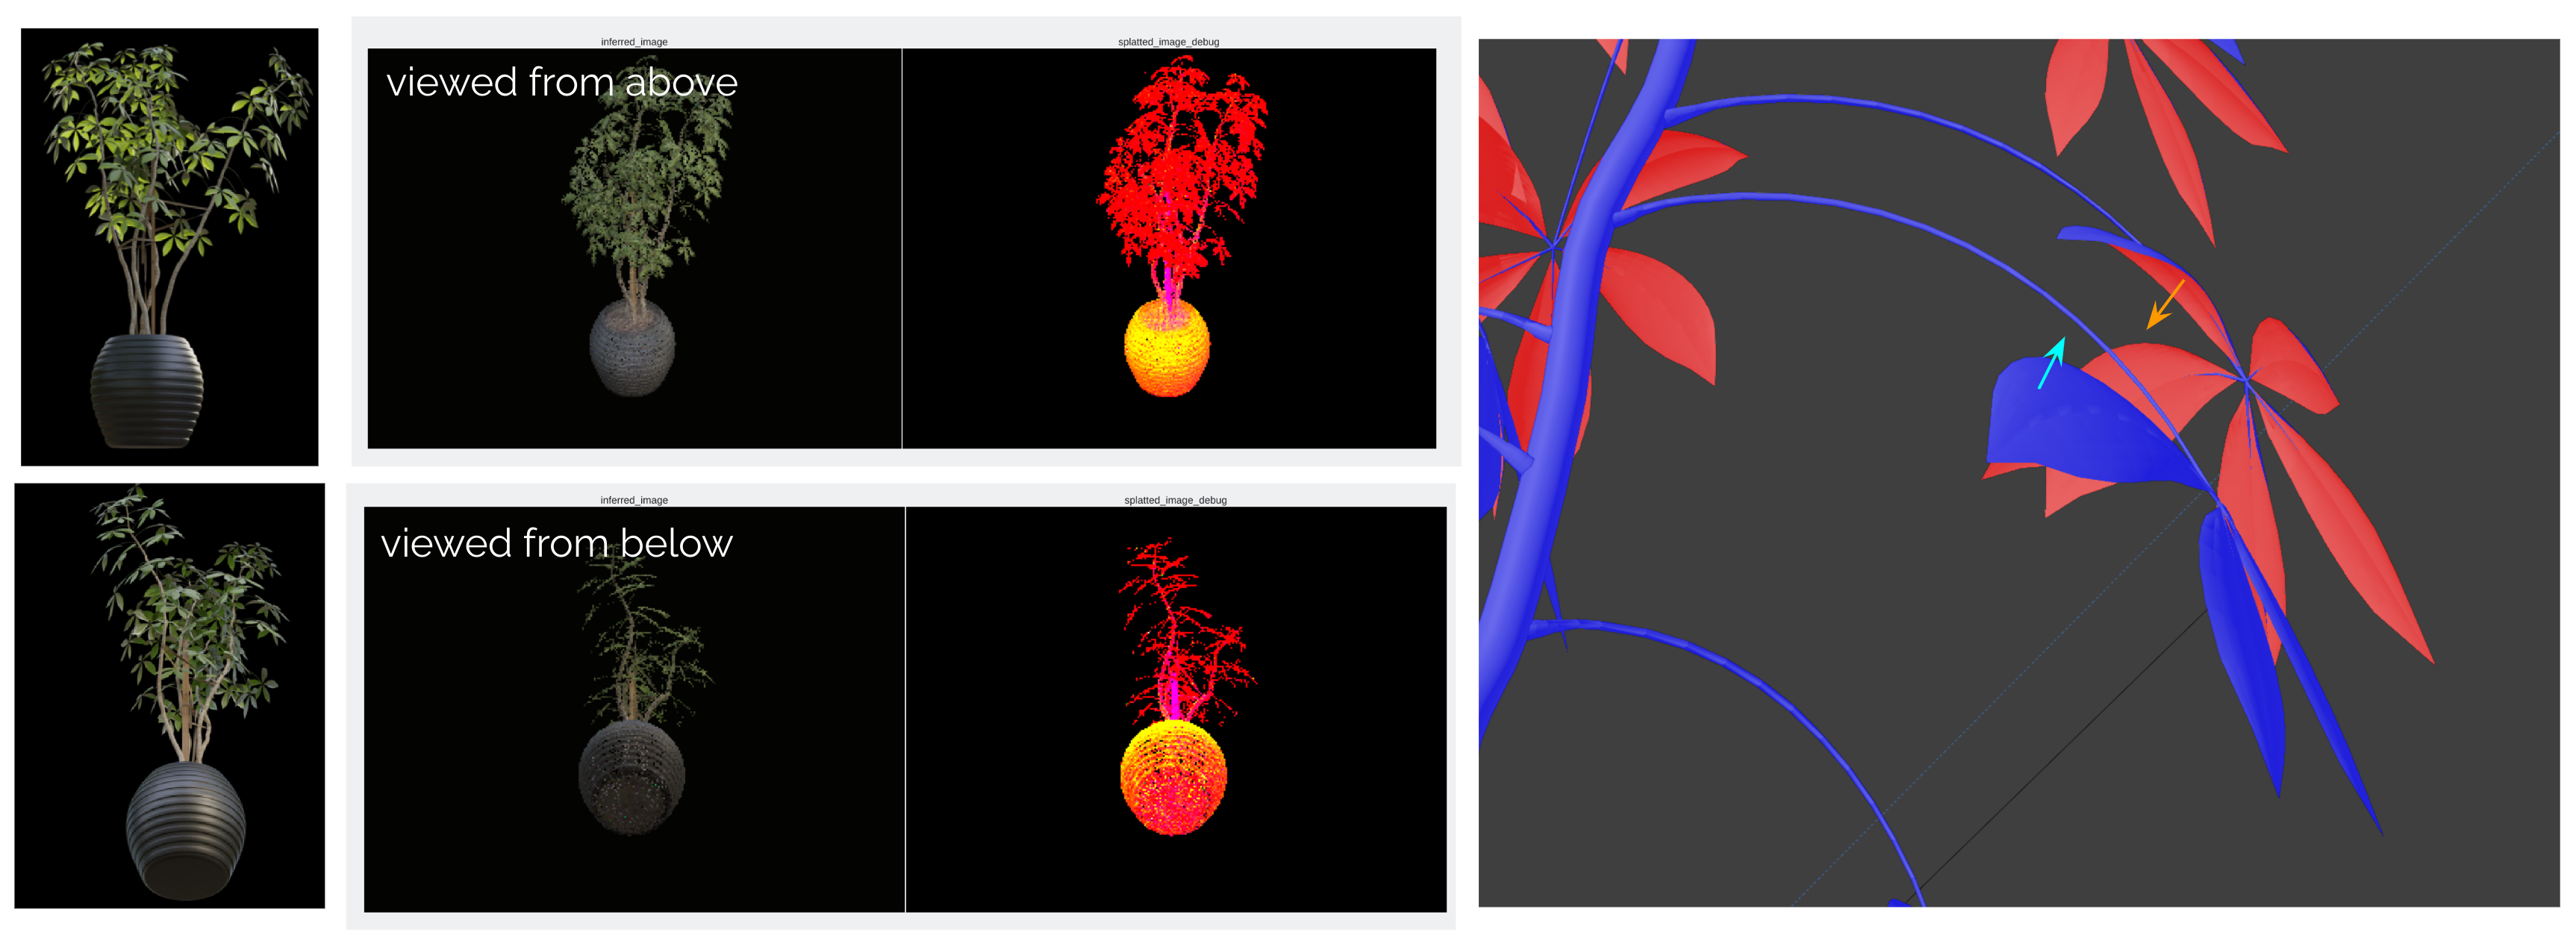
\includegraphics[width=0.8\textwidth]{figures/double_sided_surfaces_issues.png}
    \caption{On the left, image from the Blender render of the ficus scene, seen slightly from below where the leaves look brighter than when looked from above. On the right side, we check the rendering of the point cloud with the "Bypass" mode (which allows ajusting the colors points to the scene). Most leaves are oriented upwards so normal culling does not render these points when seen from below. The optimization process has trouble to reconstruct correct colors for the leaves. On the right side, the blender face orientation (blue front facing the camera/red back facing the camera) fully reveals that the leaves of the \texttt{ficus} scene are made of double sided triangles.}
    \label{fig:ficus_culling_issue}
\end{figure*}

\subsection{Projecting the point cloud onto the image plane}
\label{sec:projecting_the_point_cloud_onto_the_image_plane}

\subsubsection{Coordinates projection}
\label{sec:coordinates_projection}

\begin{figure}[H]
    \centering
    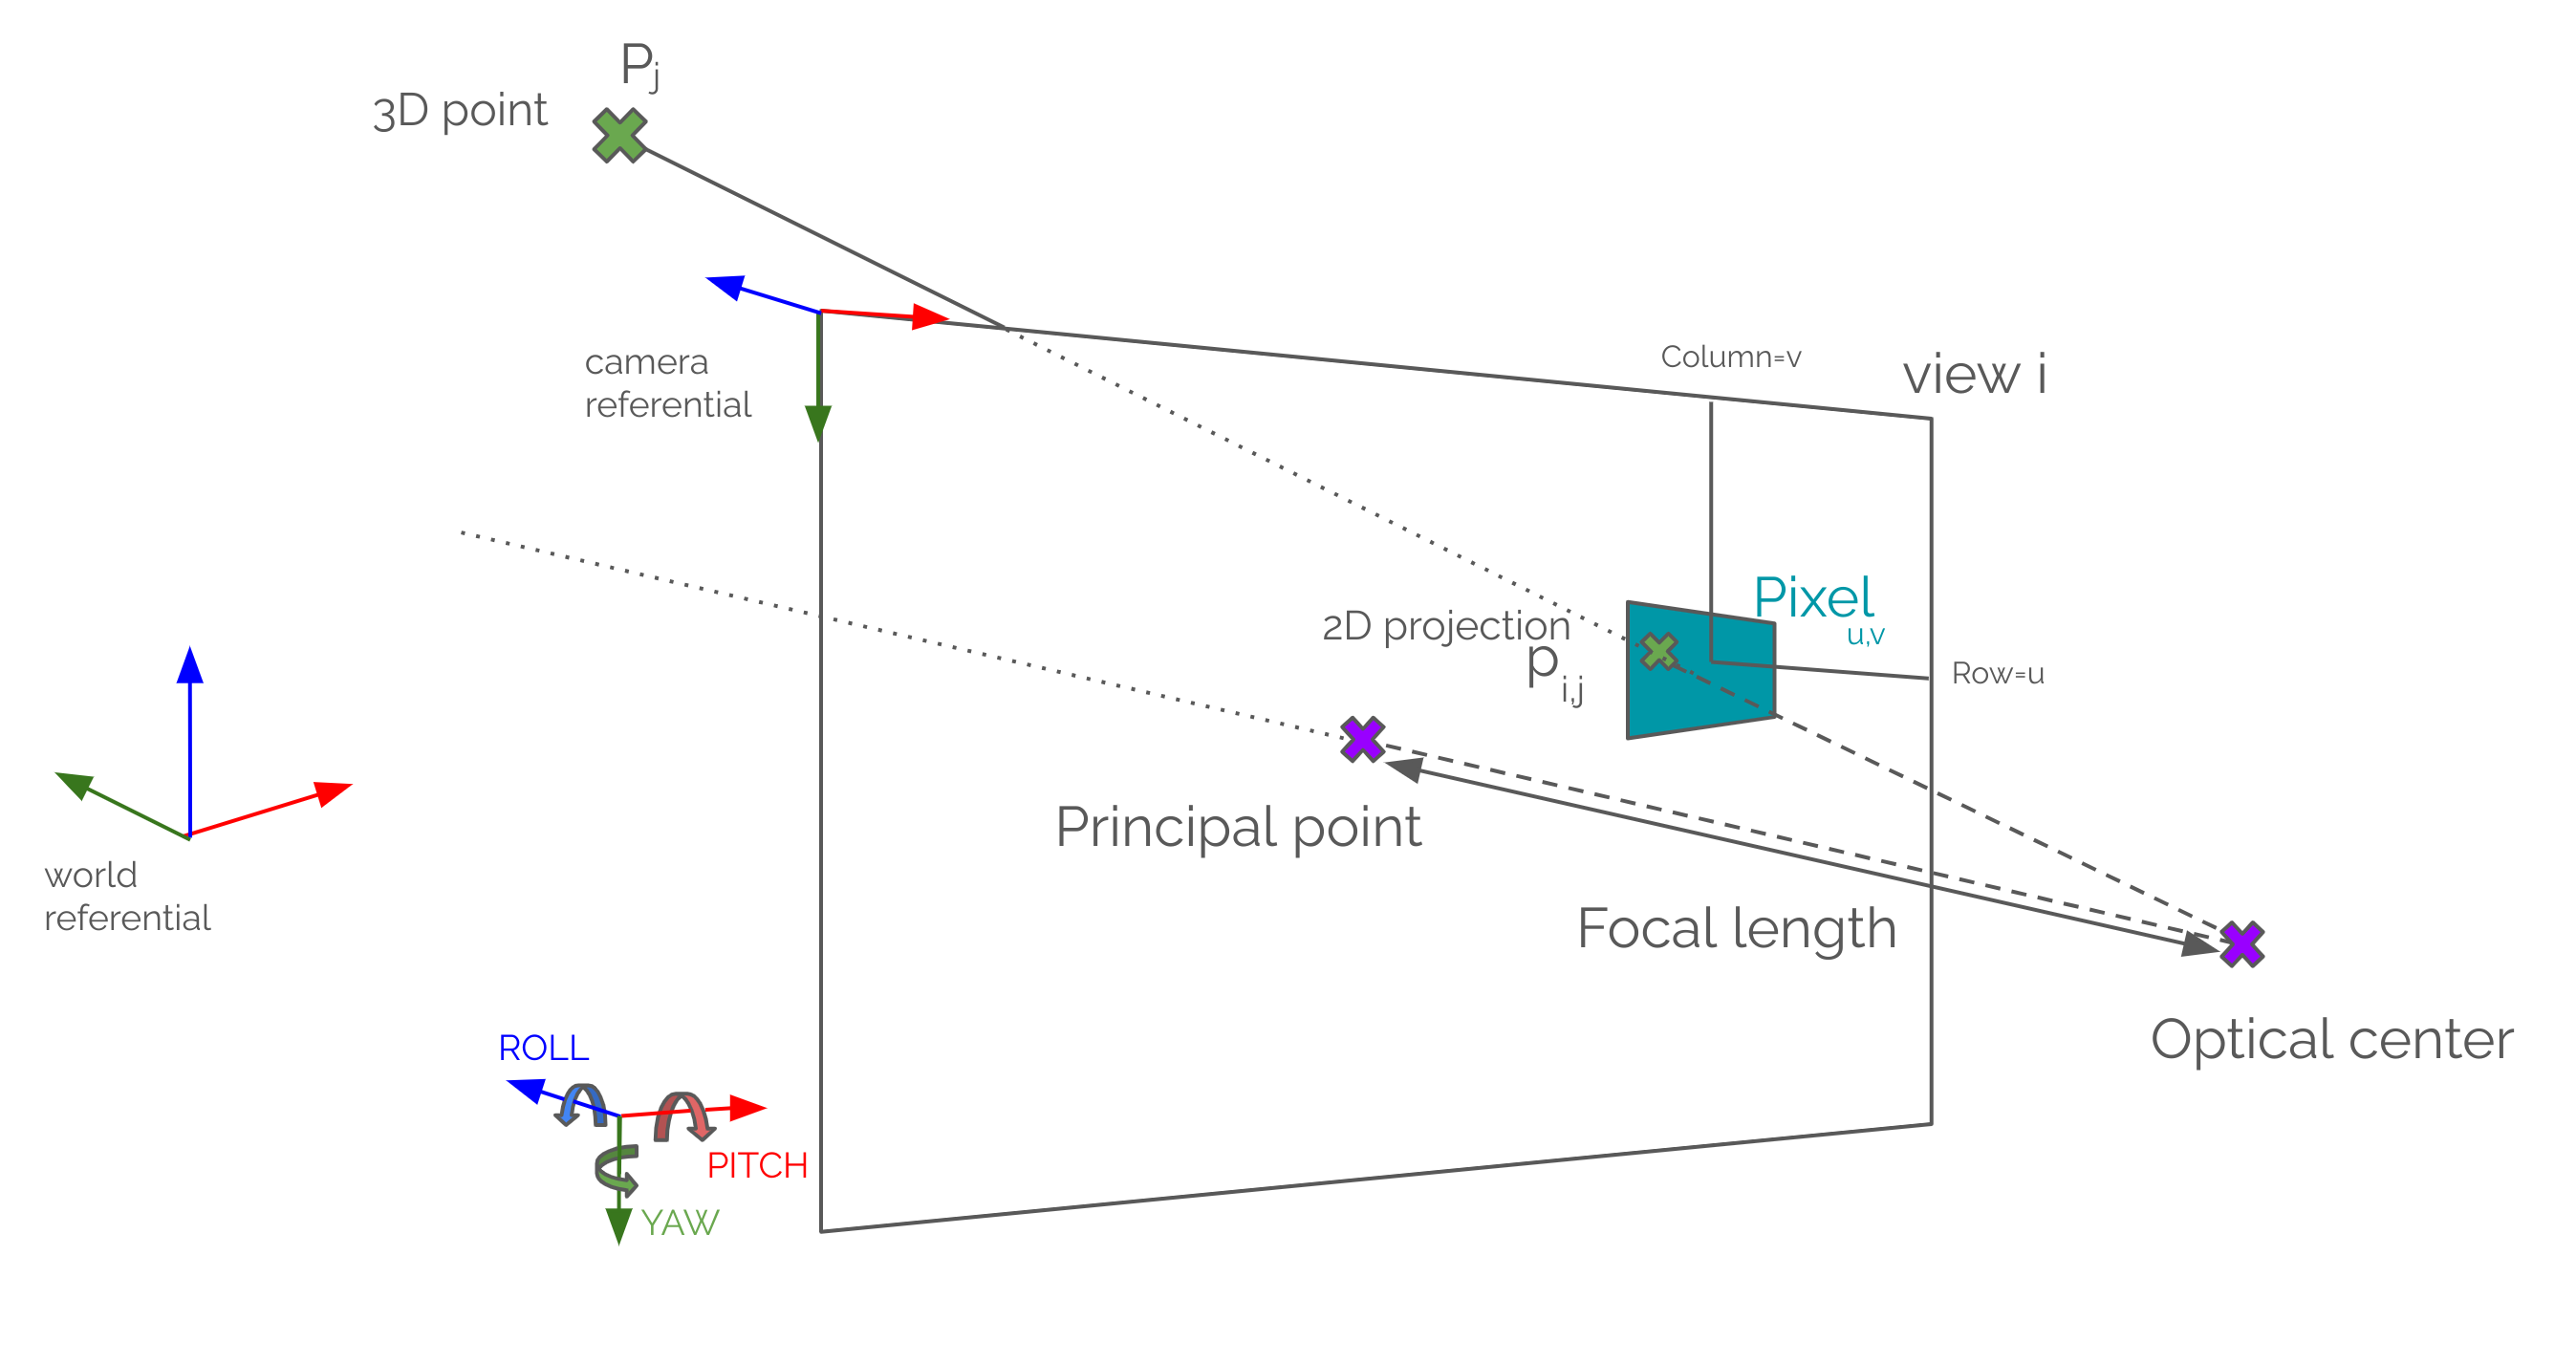
\includegraphics[width=0.4\textwidth]{figures/pinhole_camera_with_angles.png}
    \caption{Pinhole camera model. The $j^\text{th}$ point of the 3D point cloud, located at $\vec{P_{\textrm{3D}}}^{(j)}$ expressed in world coordinates is projected onto the sensor plane for view $i$ at position $\vec{p_{\textrm{2D}}}^{(i,j)}$ expressed as pixel coordinates, rounded to the 2D nearest integer coordinates $(u,v)$}
    \label{fig:pinhole_camera}
\end{figure}


To project a 3D point of index $j$ located at $\vec{P_{\textrm{3D}}}^{(j)}$ in world coordinates onto the image sensor,
we use the pinhole projection model as illustrated in \ref{fig:pinhole_camera}.

$$\vec{p_{\textrm{2D}}}^{(j)} = K\cdot\left[Q_{\text{cam}} | T_{\text{cam}}\right]^{i}\vec{P_{\textrm{3D}}}^{(j)}$$
where
\begin{itemize}
    \item $K$ is the camera 3x3 intrinsic matrix.
    \item $Q_{\textrm{cam}}^{i}$ is the camera orientation for view $i$, this matrix is created from the yaw, pitch, roll angles.
    \item $T_{\textrm{cam}}^{i}$ is the 3D camera position for view $i$ in the world frame (meters)
    \item $\vec{P_{\textrm{3D}}}^{(j)} \in \mathbb{R}^{4}$ are the homogeneous 3D coordinates of point $j$ in the world frame.
    \item $\vec{p_{\textrm{2D}}}^{(i,j)} \in \mathbb{R}^{3}$ are the homogeneous 2D coordinates of point $j$ projected in the sensor frame $i$ (pixel coordinates).
\end{itemize}

This operation is performed in ~\href{https://github.com/balthazarneveu/per-pixel-point-rendering/blob/main/src/pixr/rendering/forward_project.py}{\texttt{forward\_project.py}} in parallel over all points $j$ , using \texttt{torch.matmul} operation

\noindent \textit{Points coordinates could probably be projected all at once for all camera views using \texttt{torch.bmm}.}


\noindent \textbf{Multiscale.} Pseudocolored projected point cloud will be rendered at multiple scales. For a given scale $l \in \{0, 1, 2, 3\}$, 
$(u,v)^{(l)}$ are the rounded coordinates version of $\frac{\vec{p_{\textrm{2D}}}^{(i,j)}}{2^{l}}$.

\subsubsection{Scatter operation.}
\label{sec:scatter_op}

Visible points's colors are copied into corresponding pixels on the 2D image. A point only leads to a single pixel color update by taking the nearest pixel coordinate of $\lceil\vec{p_{\textrm{2D}}}^{(j)}\rfloor$. There are conditions to satisfy for each point to be valid. 
\begin{itemize}
    \item $(C1)$ The point must be inside the image frame $0\leq x<W$ and $0\leq y <H$.
    \item $(C2)$ The point must be in front of the camera ($Z>0$).
    \item $(C3)$ The normal of the point must face the camera - see ~\cref{fig:normal_culling_validation}.
    \item $(C4)$ The point must not be occluded by another point.
\end{itemize}

\begin{figure}[htpb]
    \centering
    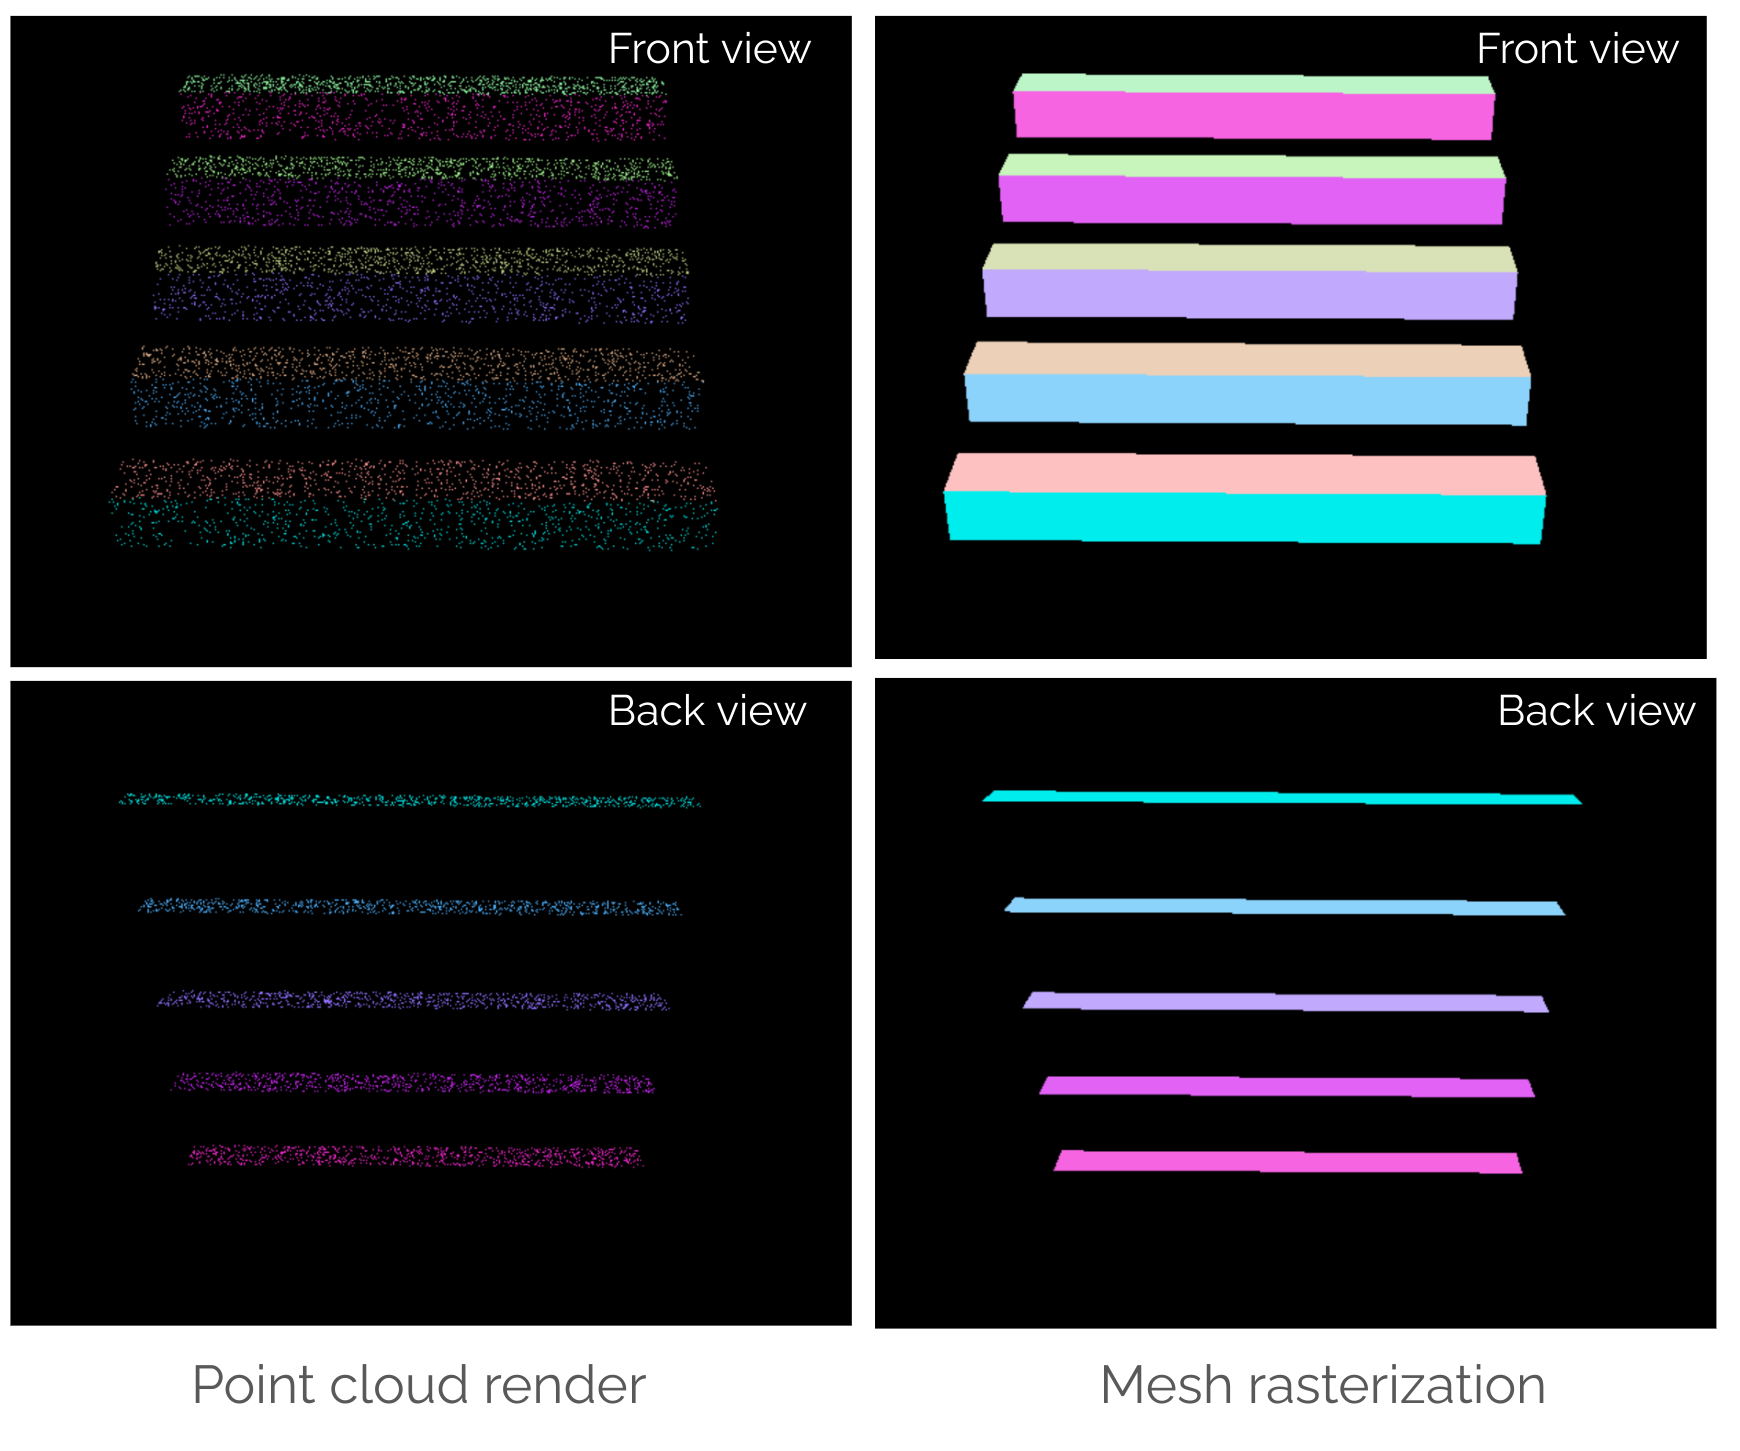
\includegraphics[width=0.45\textwidth]{figures/normal_culling_validation.png}
    \caption{Validation of normal culling. We do not render points with normals pointing away from the camera.}
    \label{fig:normal_culling_validation}
\end{figure}



\noindent \textbf{Soft depth test.} 
That last condition requires some work:
Using a Z-buffer, it is possible to take the closest point to the camera. Since several points may fall into the same pixel cell, there will be aliasing as several pixels may be located on the same suface. The authors rely on previous work \cite{schutz2021rendering} to average point colors in a tiny range of depths located behind the closest point. This is called a soft depth test and we'll describe this part in details as it required a tricky implementation with Pytorch.

\begin{figure}[H]
    \centering
    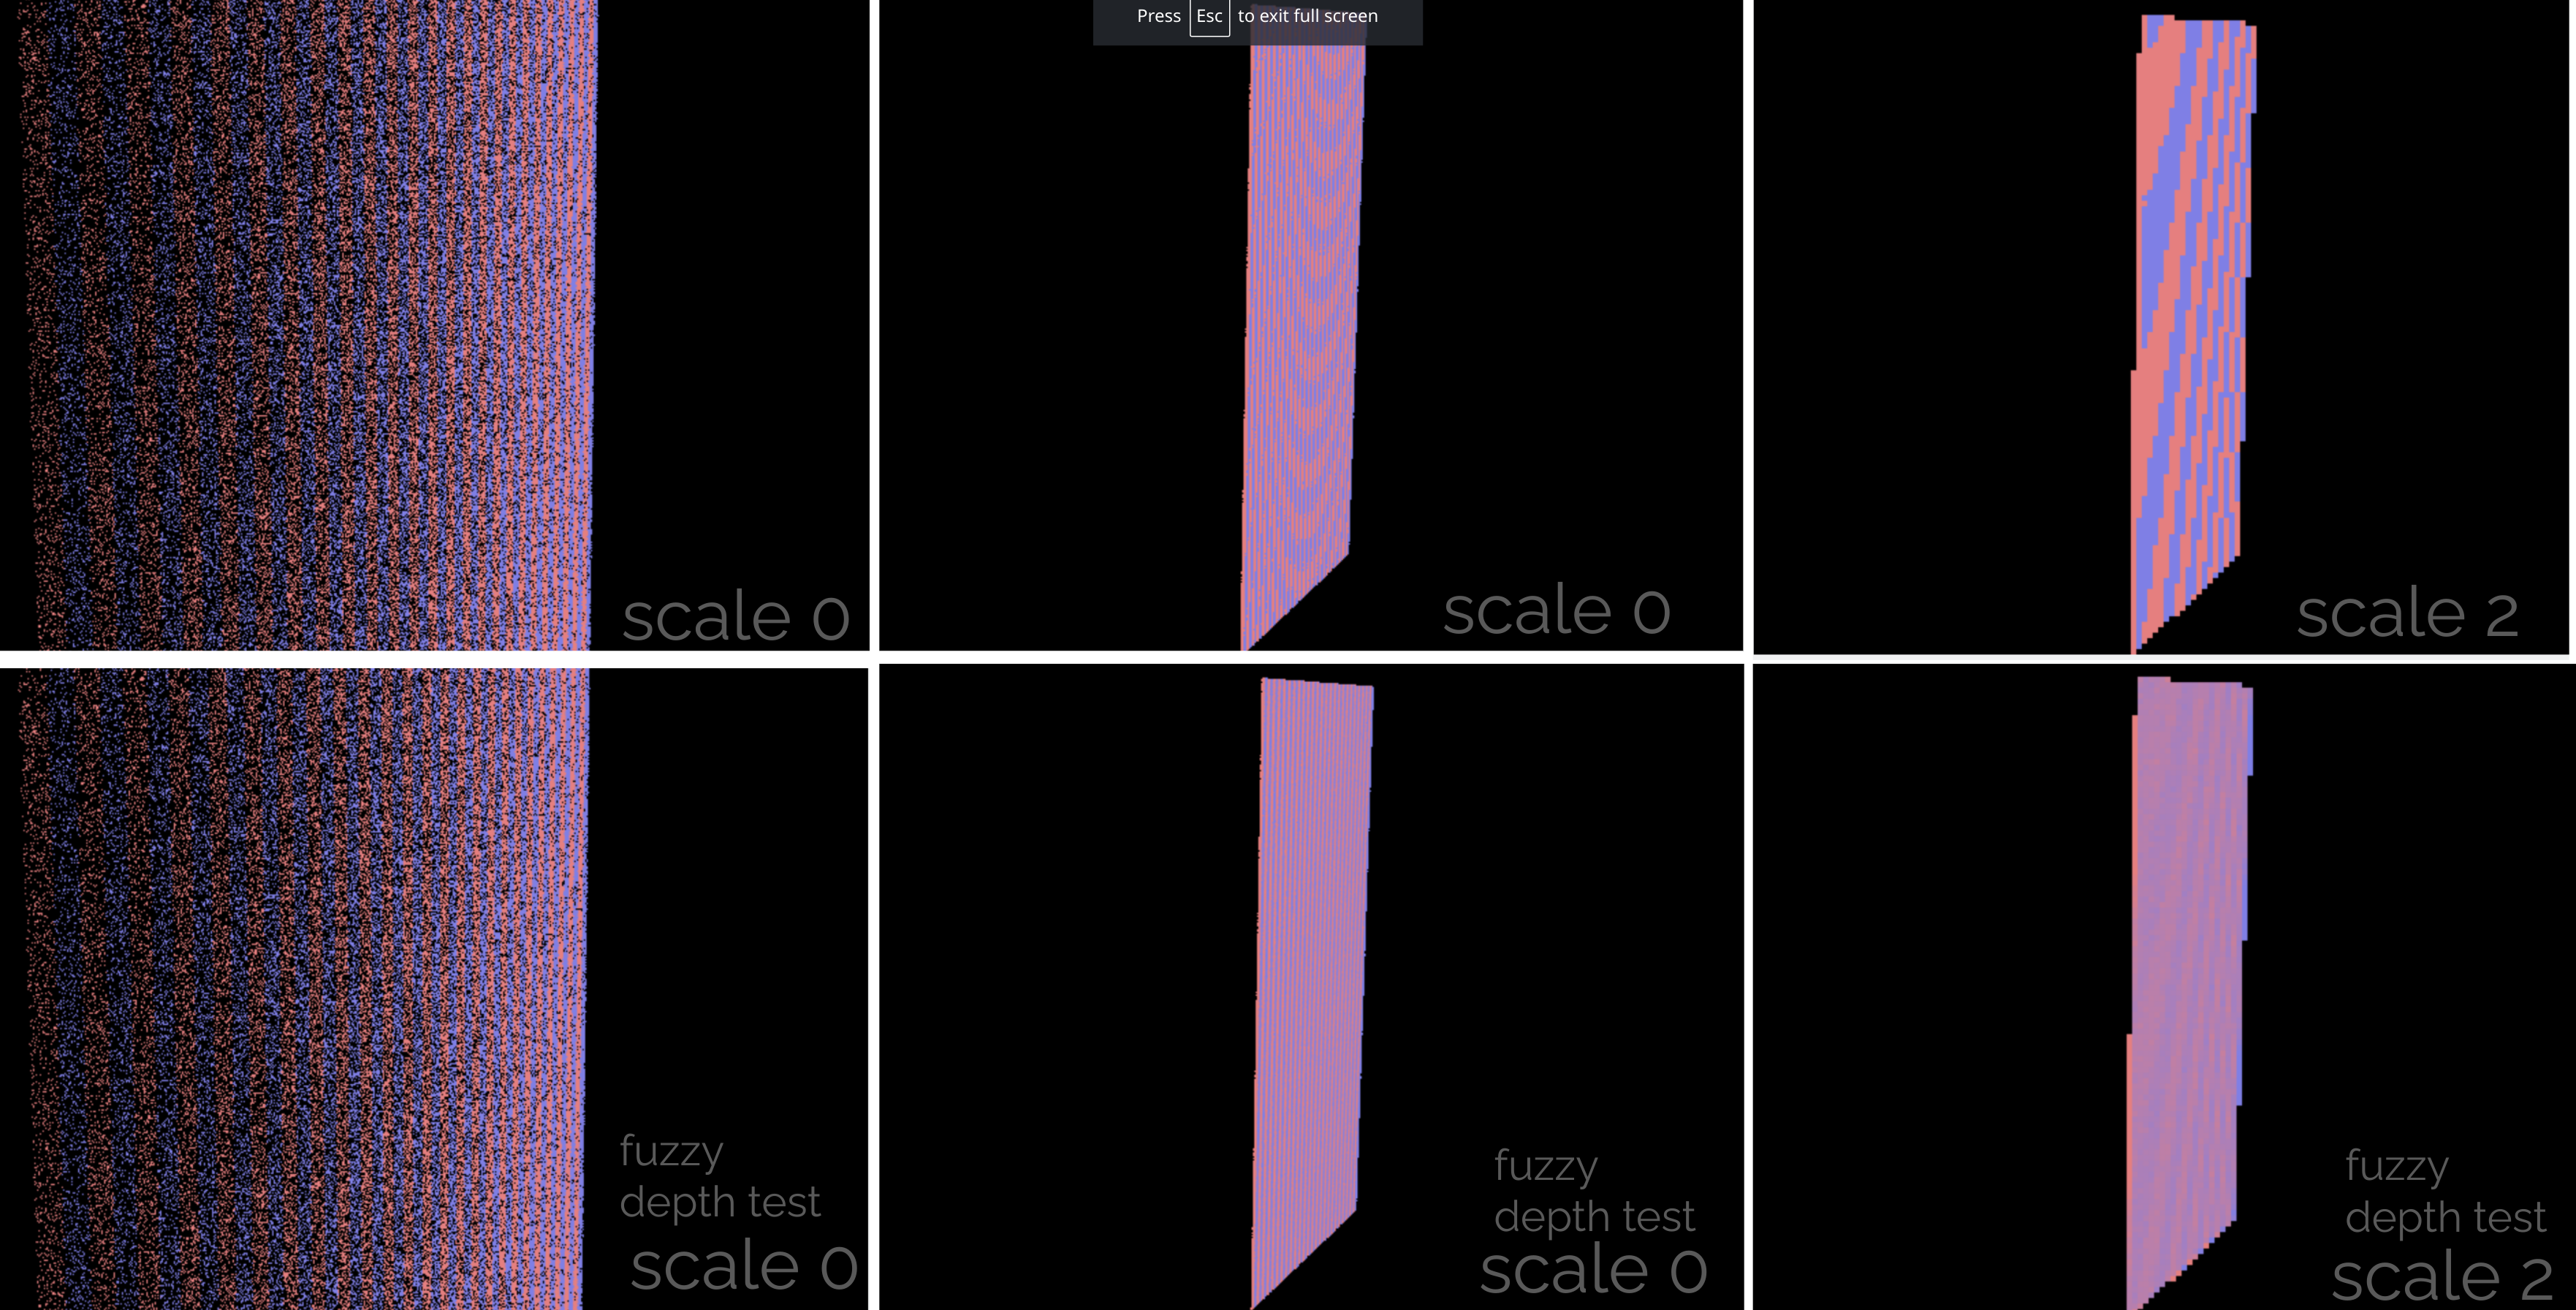
\includegraphics[width=0.45\textwidth]{figures/fuzzy_depth_test_aliasing_large.png}
    \caption{Fuzzy depth test acts as an anti-aliasing filter. On this test scene, a point cloud made of 500.000 point located in the same plane with an alternate vertical red an blue stripes on . We use $\alpha=0$ on the top (hard depth test) and $\alpha=0.01$ on the bottom (soft depth test). On the right side, when using larger scales (lower resolutions), aliasing effect if naturally amplified.}
    \label{fig:fuzzy_depth_test_AA}
\end{figure}

Soft depth test $Z \leq (1 + \alpha) * \textrm{min}_{Z_{j}}$ requires two passes. First compute the closest point to the camera for each pixel. Then, for each pixel, average the colors of the points that are close enough to the closest point. As we'll perform the first pass, we'll keep track of conditions $(C1)$, $(C2)$ and $(C3)$ to avoid recomputing them during the second pass.

\noindent \textbf{First pass: Hard depth test.}

\noindent ~\href{https://github.com/balthazarneveu/per-pixel-point-rendering/blob/main/src/pixr/rendering/zbuffer\_pass.py#L5}{\texttt{zbuffer\_pass.py}} is the first pass. It allows to find the closest point to the camera for each pixel. Depth values are initialized at $\inf$ and will remain $\inf$ when a pixel has not been filled. A first implementation trick is for each point of index $j$ to keep a linear index $k$ of its coordinate position in the image $k[j] = 1+ u*W+v$ if the point is valid regarding conditions $(C1)$, $(C2)$ and $(C3)$ and set this index to $k[j]=0$ otherwise. This allows to avoid recomputing the same test conditions during the second pass.

We then obtain the closest depth image for each pixel. $\forall (u,v) \in \left[0, H-1\right] \times \left[0, W-1\right]$:
$$Z^{\texttt{min}}_{(u,v)} = min_{\left\{j  \text{ s.t. } k[j]=1+u*W+v\right\}} \left(Z[j]\right)$$
\noindent Although this index mapping looks unnatural, it allows to use the ~\href{https://pytorch.org/docs/stable/generated/torch.Tensor.scatter\_reduce\_.html#torch.Tensor.scatter\_reduce\_}{\texttt{torch.scatter\_reduce\_}} operation to take the minimum of depth values for each pixel in a 1D tensor of size $1+W*H$.

My first ~\href{https://github.com/balthazarneveu/per-pixel-point-rendering/blob/main/src/pixr/rendering/legacy\_splatting.py}{\texttt{legacy\_splatting.py} implementation with a for loop} was way too slow and using native torch operators allowed me to get fast point cloud rendering (and save some development time to avoid rewriting a custom CUDA kernel).

\noindent \textbf{Second pass. Soft depth test and color aggregation}

In the second pass  ~\href{https://github.com/balthazarneveu/per-pixel-point-rendering/blob/main/src/pixr/rendering/colors\_aggregation.py}{rendering/colors\_aggregation.py}, we are now capable to apply the soft depth test as we have already computed the closest distance of the point cloud to the camera for each pixel. We'll modify the point index mapping $k[i]$ to only keep indices which satisfy the soft depth test: 
$$ k'[j] = k[j] * \left(Z[j] \leq (1+\alpha) *Z^{\texttt{min}}_{(u,v) \equiv k[j]}\right)$$

\noindent Multiplying by the boolean tensor gracefully sets to 0 the indices which do not satisfy the condition and keeps the others unchanged. Keep in mind that the $k=0$ index is the invalid pixel and will be discarded.
Finally, we average the colors of the points that satisfy the soft depth test, at each pixel location, using \texttt{torch.scatter\_reduce\_} operator with the \texttt{reduce=`mean`}. It is possible to keep a background

\begin{figure*}[h]
    \centering
    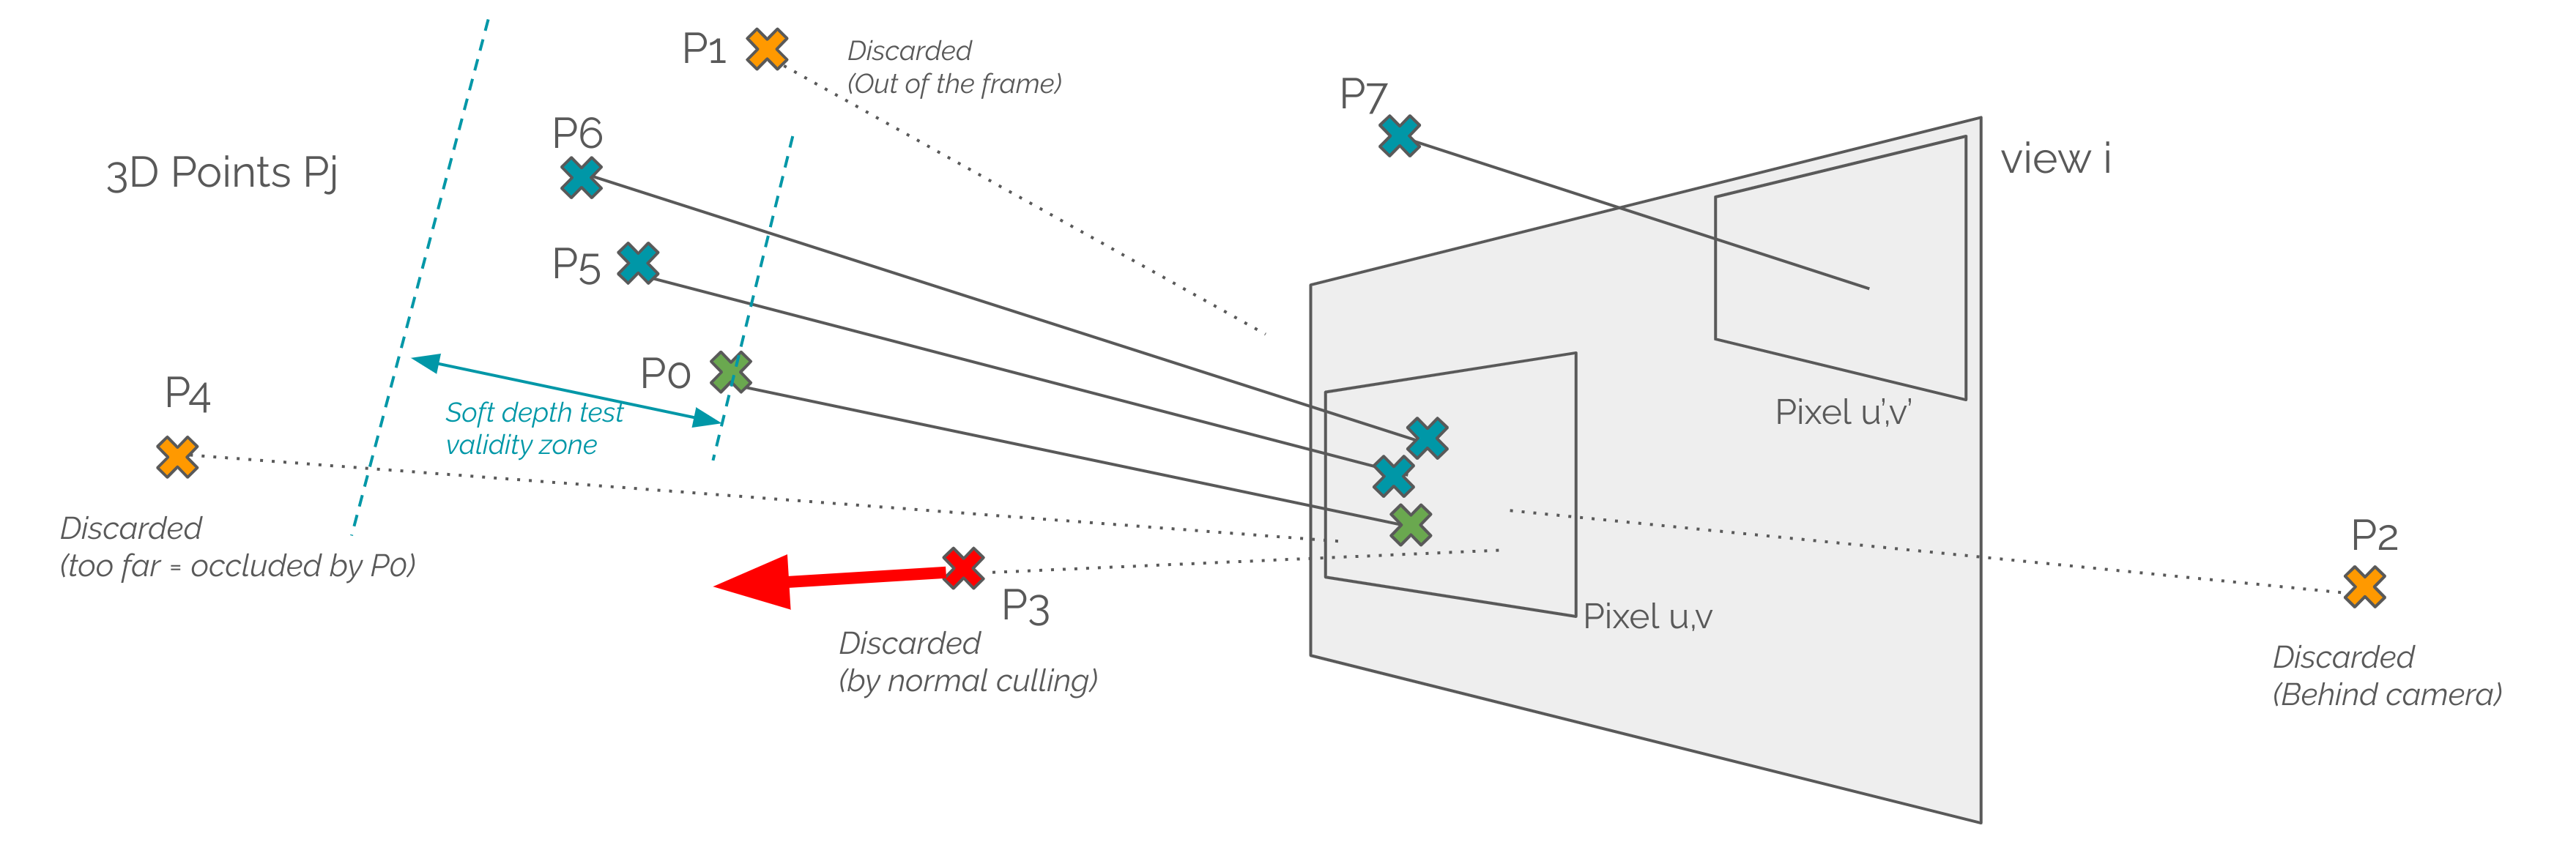
\includegraphics[width=0.9\textwidth]{figures/soft_depth_test_two_pixels.png}
    \caption{Soft depth test illustration: 
    $P^{(0)}$ is the closest point to the camera for pixel $(u,v)$. We will average the colors of the points $(P^{(0)}, P^{(5)}, P^{(6)})$. During the first pass, we'll keep track of the mapping between point indices and projected coordinates (in a 1D fashion). $k[0]=k[4]=k[5]=k[6]=1+u*W+v$ and $k[1]=k[2]=k[3]=0$, $k[7] = 1+u'*W+v'$. First pass will find the minimum of depths for each pixel $Z^{\texttt{min}}_{(u,v)} = min_{\left\{j  \text{ s.t. } k[j]=1+u*W+v\right\}} \left(Z[j]\right), \forall (u,v) \in \left[0, H-1\right] \times \left[0, W-1\right]$. For instance $Z^{\texttt{min}}_{(u,v)} = Z^{(0)}$ and $Z^{\texttt{min}}_{(u',v')} = Z^{(7)}$. \\ During the second pass, we'll only keep indices which satisfy the soft depth test: $ k'[j] = k[j] * \left(Z[j] \leq (1+\alpha) *Z^{\texttt{min}}_{(u,v) \equiv k[j]}\right)$.
   For instance, point 4 is considered too far away and discared e.g. $k[4]=0$. \\Finally, colors are averaged $I_{u, v} \propto \sum_{j \texttt{ s.t  } k'[j]=1+u.W+v}{I(j)}$. For instance $I_{(u, v)} = \frac{I(0) + I(5) + I(6)}{3}$ and $I_{(u', v')} = I(7)$.}
    \label{fig:soft_depth_test}
\end{figure*}


\subsubsection{Pixel rendering.}
\label{sec:pixel rendering}
The last operation is to render the final pixel colors by decoding the pseudo color images.
ADOP \cite{ruckert2022adop} and NBPG \cite{Aliev2020} both use a modified UNET \cite{ronneberger2015unet} which is a widely used multi-scale image processing architecture. Two modifications are made to the UNET architecture:
\begin{itemize}
    \item Convolution operator is a gated convolution proposed in a 2019 NVidia paper dedicated to image inpainting \cite{yu2019freeform}. This operator requires knowing the mask (e.g. which pixels are valid).
    \item At each scale, the UNET encoder takes pseudo-colored renders of the point cloud. Note that, at low resolution (higher levels of the pyramid), many points end up being averaged in the same pixel as described in the soft depth test. We end up with thumbnails with not much holes which will intuitively simplify rendering (this is not equivalent to downsampling the full resolution images filled with holes). 
\end{itemize}

I started implementing a Vanilla architecture shown in ~\href{fig:decoders} to make sure I could improve the point cloud rendering right.architecture in the next section. Pseudo colors have more than 3 channels (4 or 8). At the top of the pyramid ($l=3$), the projected point clould pseudo colors tensor is decoded to a tensor with 8 channels (still not a RGB thumbnail but a feature map). The lower scale $l=2$ will be processed by another decoder - but in a residual fashion (meaning that the decoded feature vector from scale $l=3$ will be upsampled and added to the feature vector of the decoder at scale $l=2$). Finally at scale $l=0$, the high resolution decoded feature map is processed by another Conv+Relu layers to end up with 3 channels. We can see on the right side that I have added an auxiliary decoder at each scale to be able to add a multiscale supervision loss (not mentioned in the original ADOP paper).
\begin{figure}[H]
    \centering
    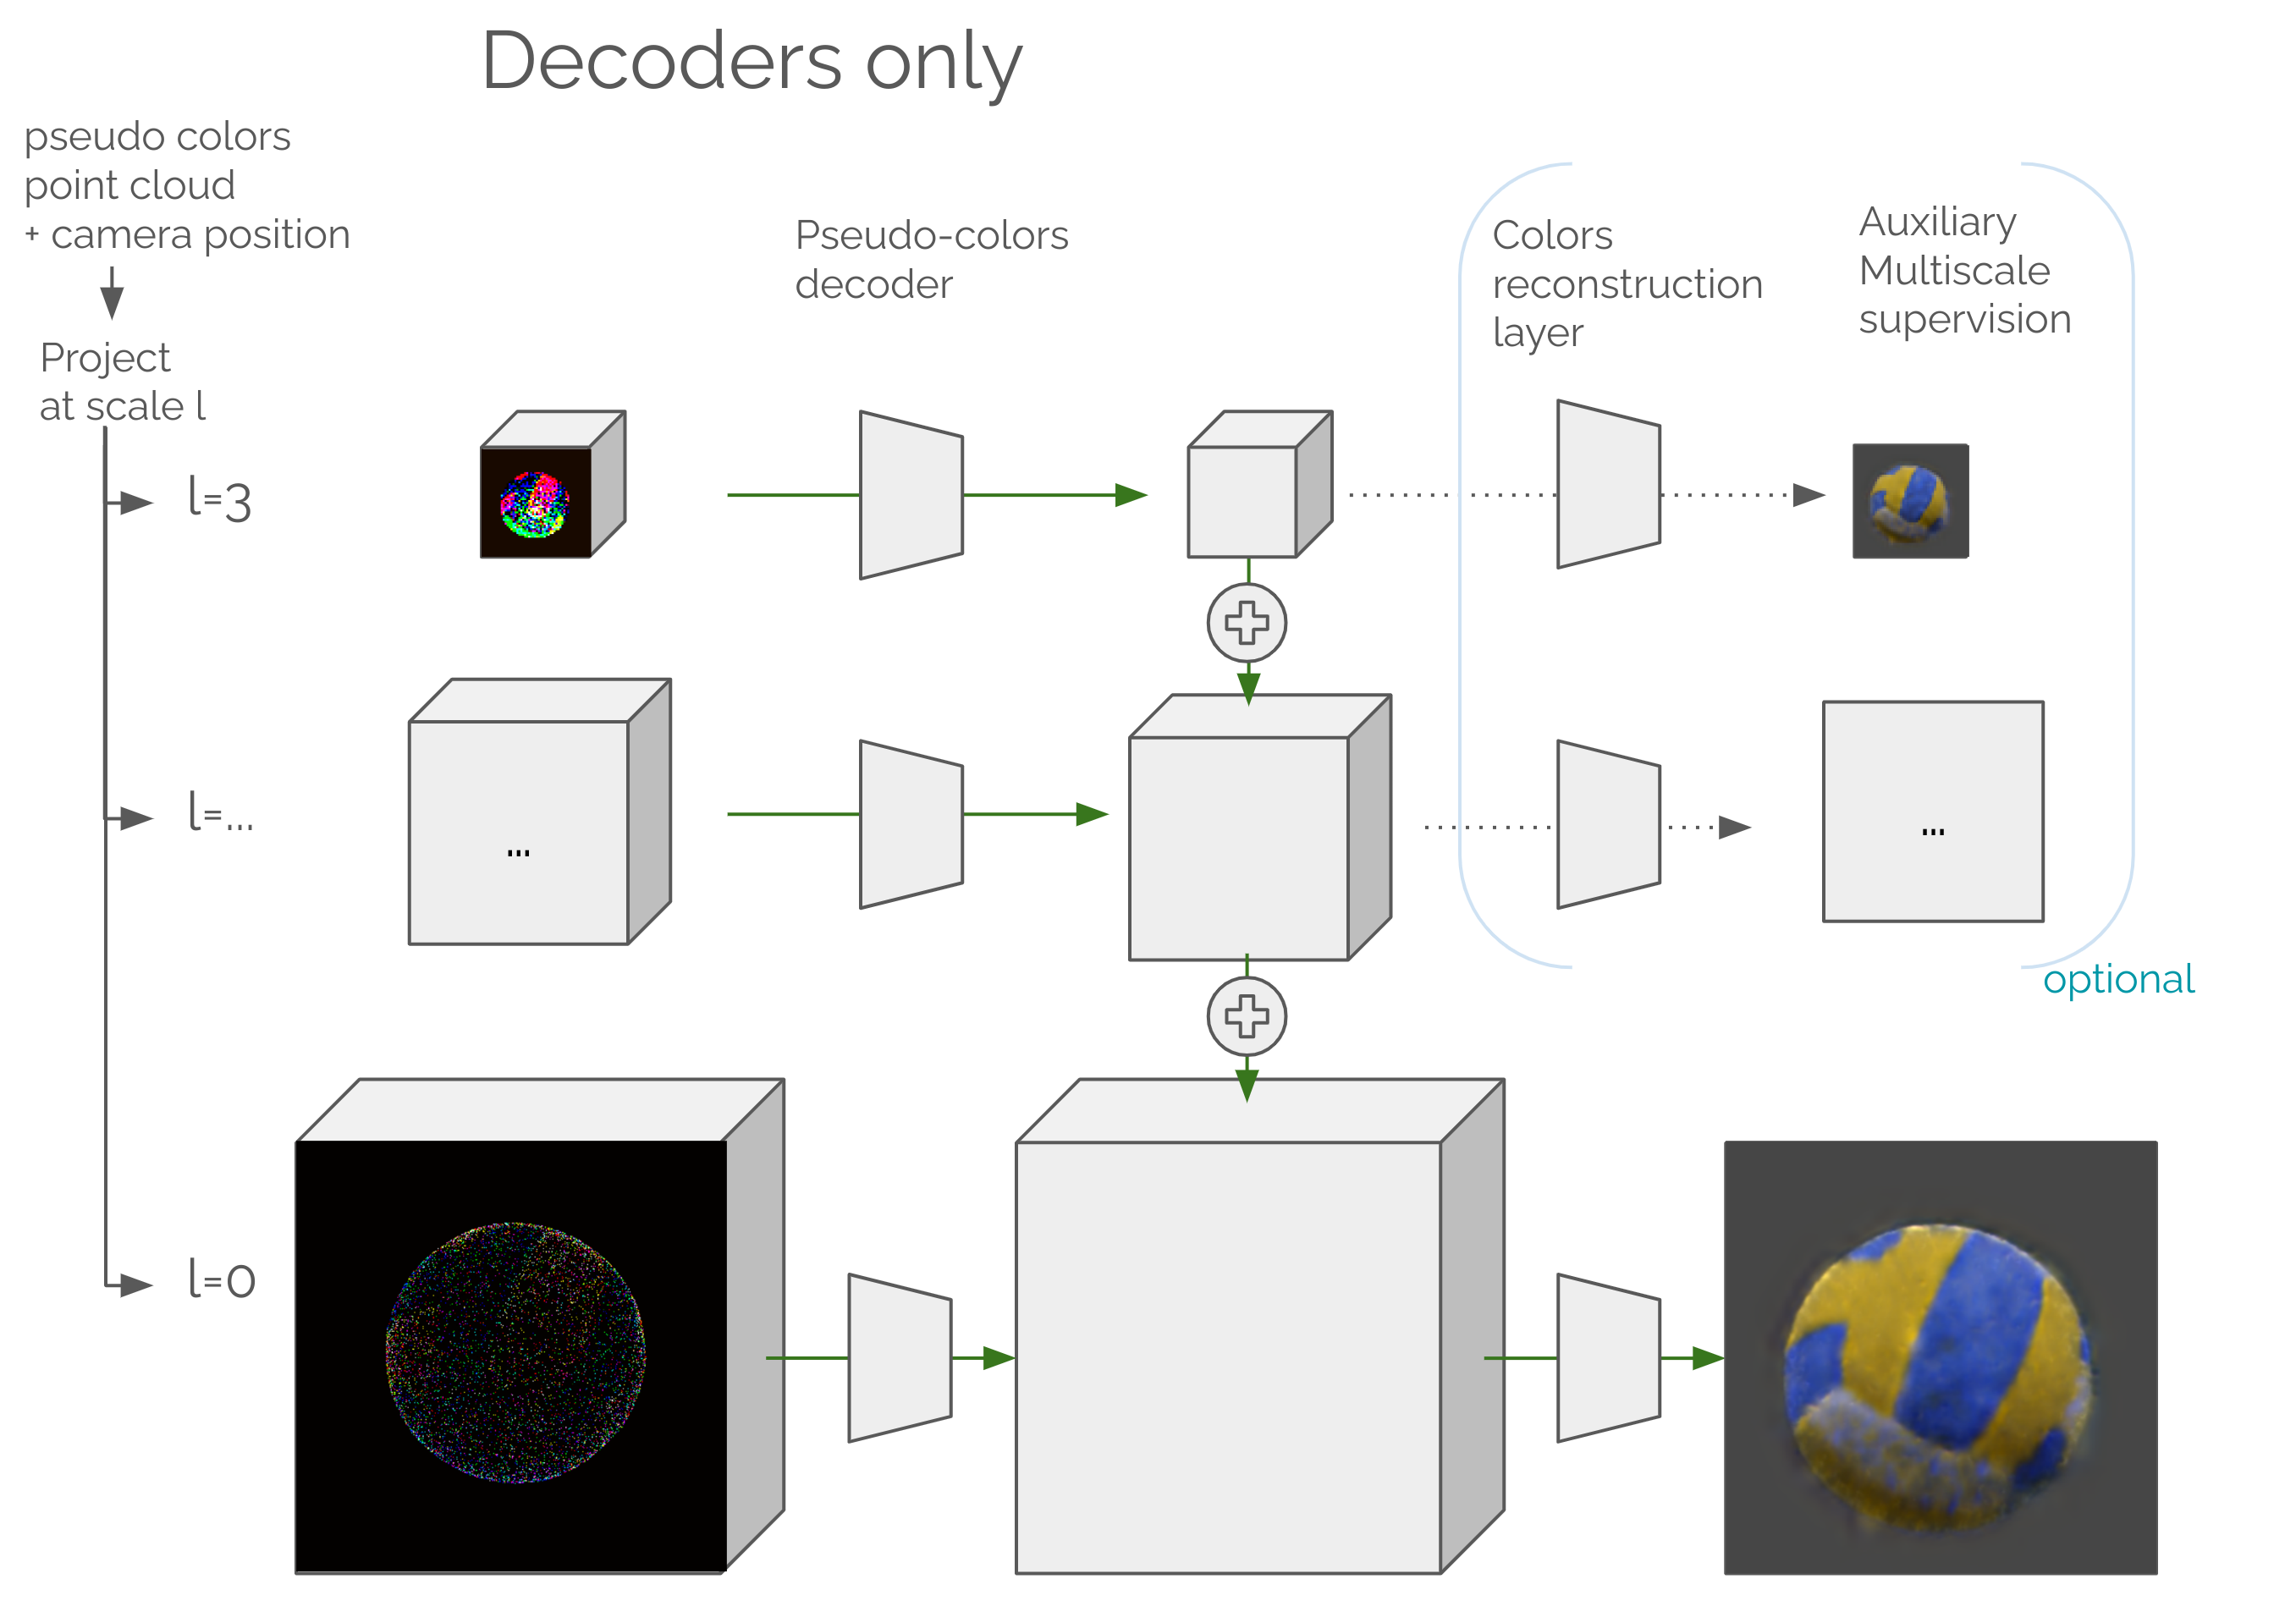
\includegraphics[width=0.45\textwidth]{figures/multiscale_decoders_only.png}
    \caption{Vanilla architecture: Multiscale CNN with decoders only. }
    \label{fig:decoders}
\end{figure}
  \section{Discussion on the original paper}
\label{sec:discussion}
ADOP\cite{Aruckert2022adop} is overall an excellent paper. It does not bring so much novel ideas but makes a considerable engineering effort to apply the core idea of NPBG \cite{Aliev2020} to large real scenes.
We'll discuss a point of criticism in the next section.\\
\noindent \textbf{~\ref{subsec:limits_real_scenes}{: Real scenes $\approx$ biased evaluation}}. Evaluation on real scenes from the Tanks and Temple dataset \cite{Knapitsch2017TanksAndTemples} mixes two things:
\begin{itemize}
    \item the inherent neural rendering method (point based rendering) quality assesment.
    \item all improvements made by taking into account the camera pipeline.
\end{itemize}
Despite ablation studies to see the effect taking the camera photo pipline into account, the comparison to other methods is unfair and I'll propose a few ideas for a new benchmark to evaluate neural rendering quality in a more controlled environment for research purpose.\\
In section ~\ref{subsec:improvement_ideas}, I will discuss some improvement ideas I had while working on the re-implementation of the ADOP paper.



\subsection{Limitation: Benchmarking only on real scenes}
\label{subsec:limits_real_scenes}
\noindent \textbf{Focusing only on real scenes.}
Suprisingly, the authors do not mention any attempts to apply their method to synthetic scenes, like the NERF paper initially did and they mention that training a new scene requires a large amount of compute. This could mean they developped their method progressively on a few toy examples and didn't bother releasing results of these tiny examples. Or their method may simply not perform too well on synthetic scenes... which may include a lot of specular materials \footnote{Classical NERF test samples scenes usually contain a lot of specular materials where the rendering would most probably fail}. I still think it would be beneficial to have a few synthetic scenes to test on including to make quick tests without the need of A100 40Gb trained for several hours.
On the other hand, since the main contribution are refining pose estimation (requiring the approximate differentiable aspect of the renderer), handling large scenes and their camera simulator, it's not surprising that the authors showcase their work on natural photos rather than simulation. 

\noindent \textbf{Camera pipeline module.}
The attempt of the authors to model the camera pipeline comes from a good intention. By including the camera pipeline as part of their rendering, they are able to: 
\begin{itemize}
    \item work in a linear color space where... performing additions or convolutions is physically grounded.
    \item compensate exposure and colors shifts per scene.
    \item get a better accuracy on the Tanks and Temple benchmark which has a lot of exposure changes.
\end{itemize}.
I think they picked the low hanging fruits here: take care of most exposure changes to end up improving the metrics on the available benchmark: Table 4. from their paper shows that ADOP is better by a large margin than all other algorithms (except the M60 tanks scene which has been shot in manual frozen exposure). 
They didn't backport their idea to the comcurrent methods they compare to so I don't think the comparison is really fair (the point based method may simply not be the key element leading to good results).

Anyway, their claim to handle the camera imaging pipeline properly and adapt to it is legitimate, well crafted and justified in the paper. But it has a major caveat: results may crumble in case of a more complex or different camera ISP \footnote{Image Signal Processor} than the one from Sony A7SII or DJI X5R.
Please refer to ~\cref*{fig:ISP}

\begin{figure*}[h]
    \centering
    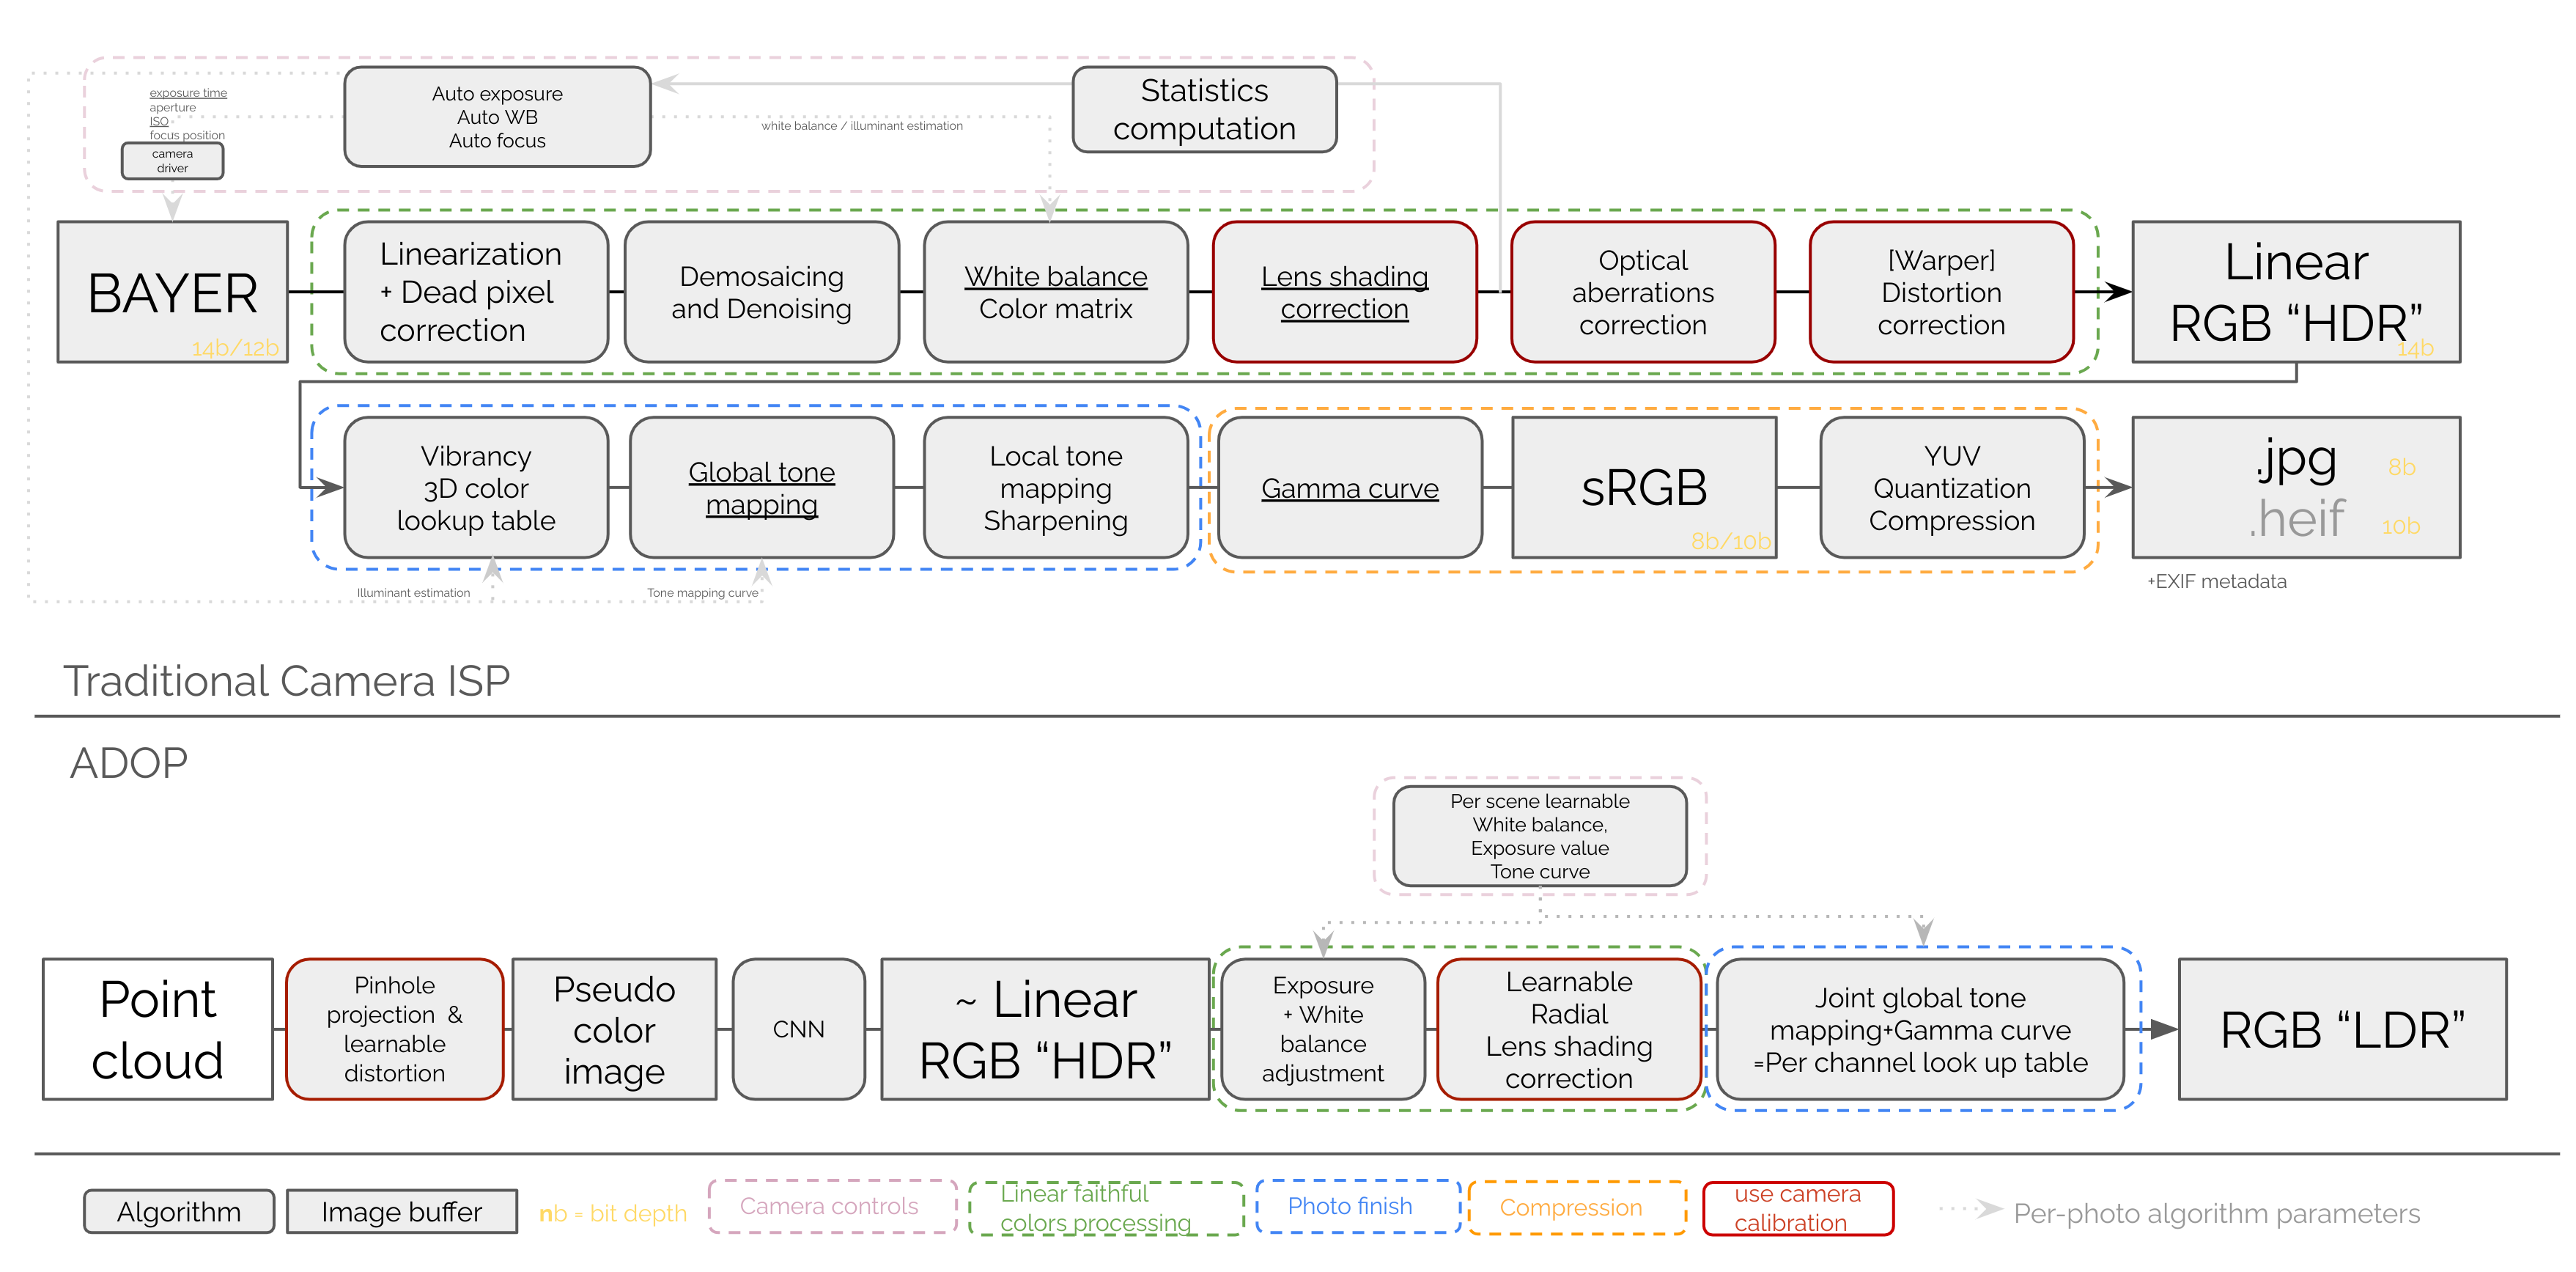
\includegraphics[width=0.9\textwidth]{figures/isp_pipeline_VS_ADOP.png}
    \caption{Comparing a modern ISP camera pipeline at the top versus the ADOP pipeline at the bottom which includes some learnable parameters such as the tone mapping curve, exposure compensation or white balance adjustments.}
    \label{fig:ISP}
\end{figure*}

Ablation study from the authors (table 3 and figure 6 of \cite{Aruckert2022adop}) shows that ADOP results get better when including the camera module in the pipeline. problem is that we don't really know the exact impact of compensating the camera photo pipeline on the final result, at least compared to a scene imaged with perfect ideal linear HDR camera.

If we carefully look at the Tanks and Temples dataset \cite{Knapitsch2017TanksAndTemples}, pictures are frames extracted from a mp4 video from 2 different high end cameras, sometimes using auto-exposure (see ~\href{fig:tank_and_temples}). Although it's a good initiative for researchers to keep on using fixed established benchmarks, Tanks and Temples was initially designed for 3D reconstructions (e.g. evaluate performances of Structure from motion like COLMAP estimation compared to a groundtruth lidar captured point cloud) rather than novel view synthesis. The idea is interesting but it will most probably fail with a modern smartphone camera which use local tone mappers and sometimes adapt colors locally. For instance, they're able to get a sky with cyan shift which looks like the camera picture (they fit the tone mapper correctly). Modern smartphone ISPs manufacturers have worked on this "cyan cast" problem (compress blue highlights instead of clipping when applying white balance) so compensating these algorithms will become harder and harder as they get more and more sophisticated.


\begin{figure}[H]
    \centering
    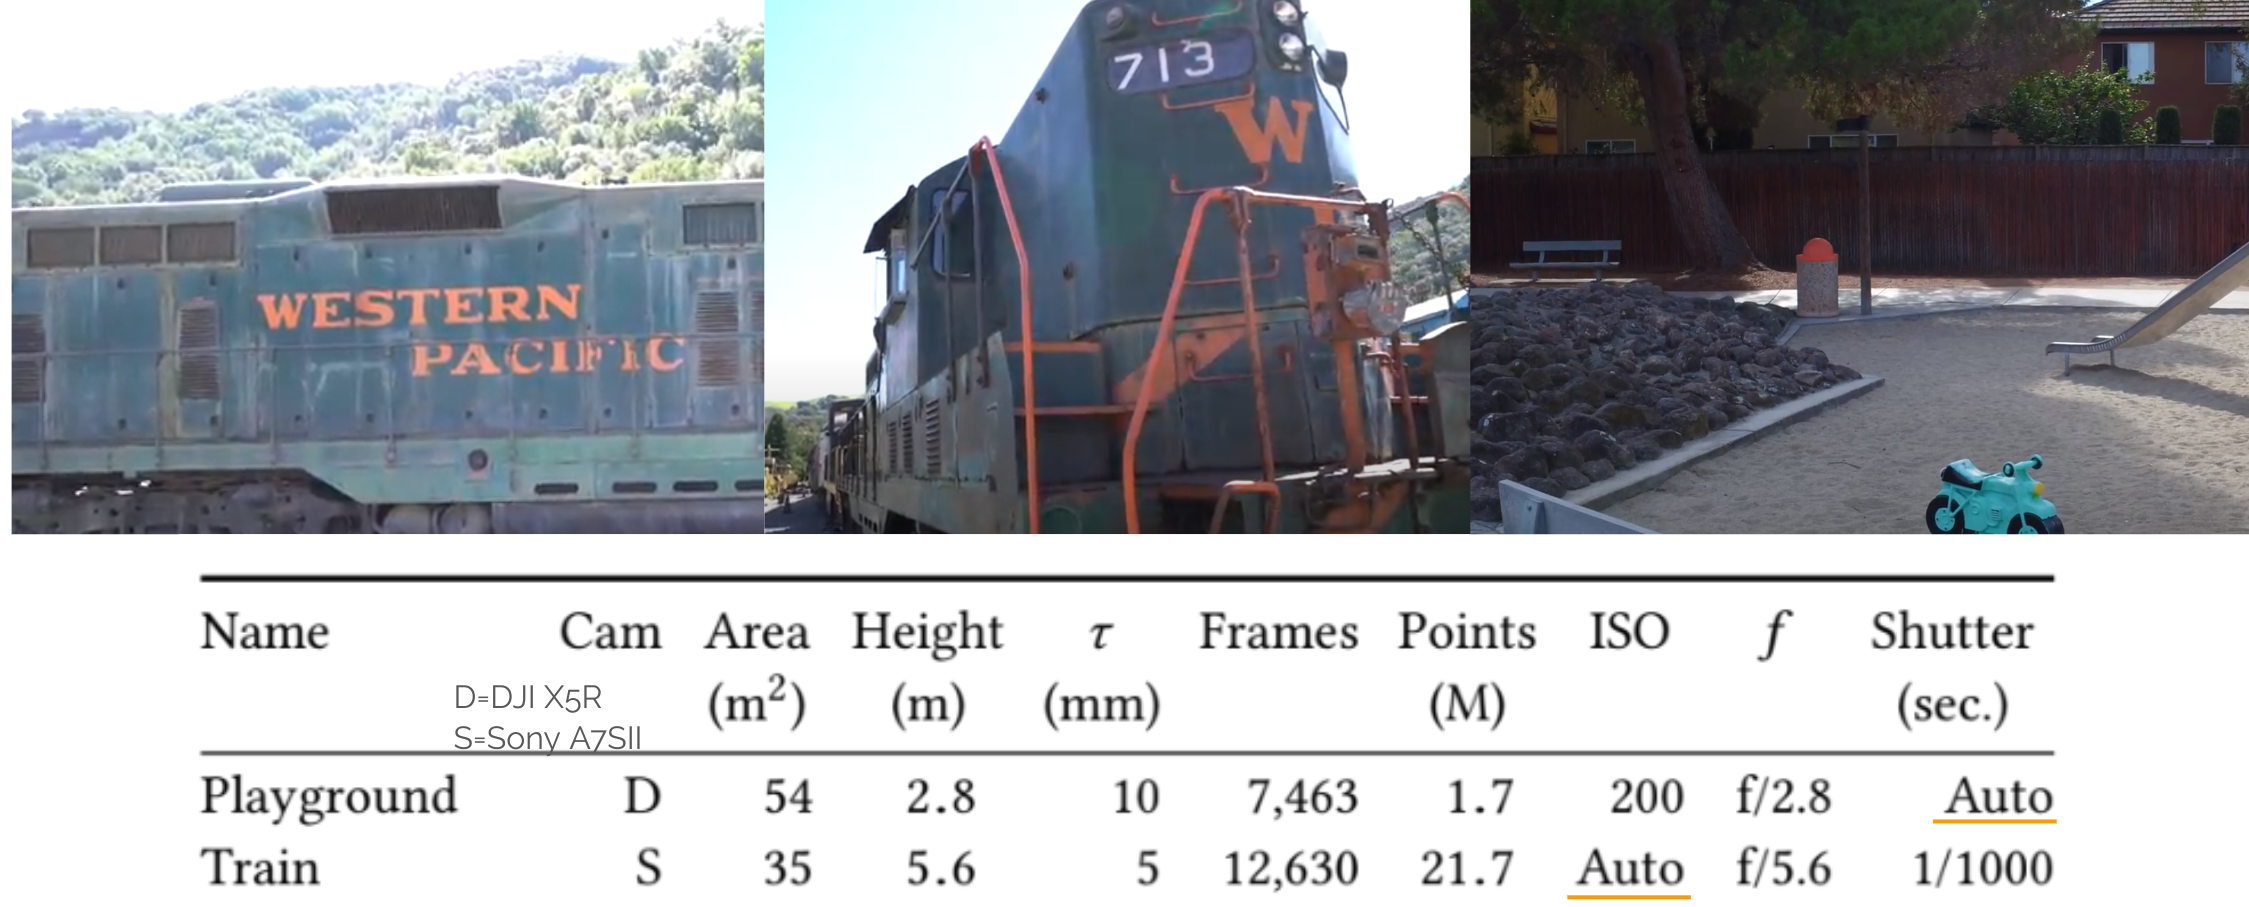
\includegraphics[width=0.45\textwidth]{figures/tanks_and_temples.png}
    \caption{Information on the scenes captured for the Tanks and Temples dataset with high end video cameras in addition to a Lidar point cloud. On the left, the "train" scene shows clear signs of overexposure. The playground scene on the right has an overall correct and steady exposure.}
    \label{fig:tank_and_temples}
\end{figure}


My recommendation is that all evaluations better be led in the linear domain. It is the best way to go make fair comparisons between novel view synthesis algorithms. Benchmarking would strongly benefit from an "upgrade":a sort of \textit{"Linear Tanks and Temples"} carefully crafted by taking RAW shots with a high end DSLR. This is proposed next.

\noindent \textbf{Switching to RAW format?} 
One of the potential way of creating a new benchmark would be to capture the scenes with a DSLR (like a full frame sensor) shot both in RAW and jpg (usually available on most cameras). RAW files would be post-processed by Adobe LightRoom or DxO Photolab with a neutral rendering: no tone mapping and neutral color rendering to get a Linear RGB set of images without any image compression. In case the sensor 12 or 14bits dynamic range is not sufficient, HDR captures could be achieved by bracketing. Intuitively, it sounds natural to use a tripod and merge the LDR linear images into a HDR linear image. But even handheld, all raw captures at various exposures could be used (let the alignment of bracketing images be implicitly done without any explicit need to merge exposures). These HDR images may serve as the ground truth for validation.

The main caveat of using RAW images is that there'll always be \textbf{noise} present proper to the camera sensor in the raw files. Since you get multiple views of the same scene, we can use the key concept proposed in Noise2Noise \cite{lehtinen2018noise2noise} that a neural network can be trained to denoise images without a ground truth images (it requires noisy burst of the same image instead). Here we have access to the same scene under different angles. The engine to implicity align them and get the right supervision is the rendering of the point cloud itself! The idea of using NERF to work on RAW data has been proposed in "NERFs in the dark" \cite{mildenhall2022rawnerf}.


RGB (raw demosaicked) linear format is the only space in which an evaluation of the rendering quality does not depend on the camera ISP.
If one would really like to check the effect Training images could be either the jpgs or the reprocessed RAW files using a more scenic rendering: vibrancy to make some colors slightly more saturated (e.g. blue for skies but avoid saturating red too much for skin tones), tone mapping (global or local), sharpening / micro contrast.



\subsection{Improvement ideas}
\label{subsec:improvement_ideas}
A lot of my implementation work has been based on trying to apply the concepts of the ADOP paper to calibrated scenes. I think that it is possible to make these photorealistic images look more like the ones we'd get from real cameras.

\subsubsection*{Calibrated scenes + realistic simulated camera pipeline}.
\noindent Regarding my simplified implementation, I did not try to include the camera pipeline module not only because of limited time but also because simulating a realistic camera pipeline is a very difficult task.
For calibrated scenes, to mimick a realistic camera pipeline, one would have to:
\begin{itemize}
    \item output HDR linear images out of Blender (\textit{BlenderProc does not even offer EXR outputs at the moment}).
    \item mimick RAW files: inverse the "blue linear" blocks of figure ~\cref*{fig:ISP}. The idea of reversing the ISP has been proposed in \cite{brooks2018unprocessing}: apply inverse white balance and color matrices from typical values, mosaick, add realistic poisson+gaussian noise depending on sensor characteristics and ISO value...
    \item Mimick the ISP which goes from 12/14bits linear RAW bayer data to a 8 bit jpg (which is a difficult task). One could simply use a high end software raw converter by re-introducing a DNG as input to Darktable (open source) or Adobe LightRoom. Another way is to use a deep neural network proxy of a blackbox ISP (see the work \cite{ignatov2020replacing} which mimicks the Huawei P20 ISP)
\end{itemize}
This is definitely \textbf{a large chunk of work} but it could bring a lot of value if one wants to try to make a commercial product for novel view synthesis which can adapt to all sorts of cameras.

\subsubsection*{Pseudo colors intialization}.
Instead of initializing the pseudo colors of each point randomly, a trick could be to pre-train an auto-encoder on the reference images. For each point in the point cloud projected onto a given view, we have a target patch in the reference view. This patch could simply be encoded into a latent vector which could be aggreagated in the pseudo-color vector. Pushing the idea further, the pretrained decoder (from the auto-encoder) coud be used as the decoder in the neural rendering network. Here's the intuition: the neural render encoder is the identity, this is kind of equivalent to copy pasting the decoded patches at the right locations.


\subsubsection*{Inherent limitations to model view dependant material appearance}.
By construction, the ADOP pipeline does not have a natural ability to model view dependent effects such as specularities or reflections. We have observed this in ~\cref{fig:material_changes} and there's no  
We could provide extra inputs to the neural network to model view dependent materials. By providing the angle between the point normal and the view direction (these 2 vectors are computed during the normal culling test). These 2 angles could be concatenated to the projected pseudo colors vectors (and we'd probably need to map these to sine positional embeddings as proposed in NERF  \cite{mildenhall2020nerf}). \textit{I eventually found out about NPBG++ \cite{rakhimov2022npbg}}. The authors of NPBG++ propose to fit the coefficients of spherical harmonics function which model color variation of each point with regard to relative camera operation.

\subsubsection*{Limitation when zooming too much}.
The inherent limitation of point appears when you zoom in too close. A continuous parametric representation \cite{kerbl3Dgaussians} such as an anisotropic 2D Gaussian Kernel would allow mixing the advantage of point clouds (scale and speed) while trying to remove their discrete nature... 
  \section{Conclusion}
\label{sec:conclusion}

In conclusion, the review of this paper has been a great opportunity to dive into the world of neural rendering and understand the challenges of point based rendering.
I have implemented two major topics: 
\begin{itemize}
    \item A script to render calibrated scenes which are ready for neural rendering (with perfect normals, perfect point cloud position and camera poses). 
    \item A pytorch implementation of point projections with the fuzzy depth test (which was satisfying - it allows perfoming live inference)
\end{itemize}
I have pointed out: 
\begin{itemize}
    \item a minor criticism regarding all tricks deployed to model the camera pipeline instead of truly questioning the relevance of benchmarks on the Tanks and Temple dataset. 
    \item a limitation regarding handling view dependent effects which is not a problem in NERF.
\end{itemize}

The amount of work spent by the authors to make their method work very fast on large scale point clouds is tremendous. The crafstmanship of the computer graphics research community is very inspiring.




  %% APPENDIX

  
  % \newpage
  \newpage

  %% BIBLIOGRAPHY
  \bibliographystyle{ACM-Reference-Format}
  \bibliography{references}

  \newpage
  \appendix
  % \section{Appendix}


\begin{table*}[htpb]
    \begin{tabular}{|l|l|l|l|l|l|}
    \hline
    Number of points & PSNR   & Mode     & Conv size & Pseudo color dimension & Multi-scale supervision \\ \hline
    100k             & 16.7dB & Bypass   & 1x1               & 3                      & Yes                     \\ \hline
    100k             & 21.2dB & Conv 5x5 & 5x5               & 3                      & Yes                     \\ \hline
    100k             & 26.3dB & Vanilla  & 5x5               & 8                      & No                      \\ \hline
    100k             & \textbf{29dB}   & Vanilla  & 5x5               & 8                      & Yes                     \\ \hline
    400k             & 23dB   & Bypass   & 1x1               & 3                      & No                      \\ \hline
    800k             & 25db   & Bypass   & 1x1               & 3                      & No                      \\ \hline
\end{tabular}
\caption{Quantitative performances (PSNR on validation set) of various training configurations on the \texttt{Old chair} scene.}
\label{tab:results}
\end{table*}


\begin{figure*}[htpb]
    \centering
    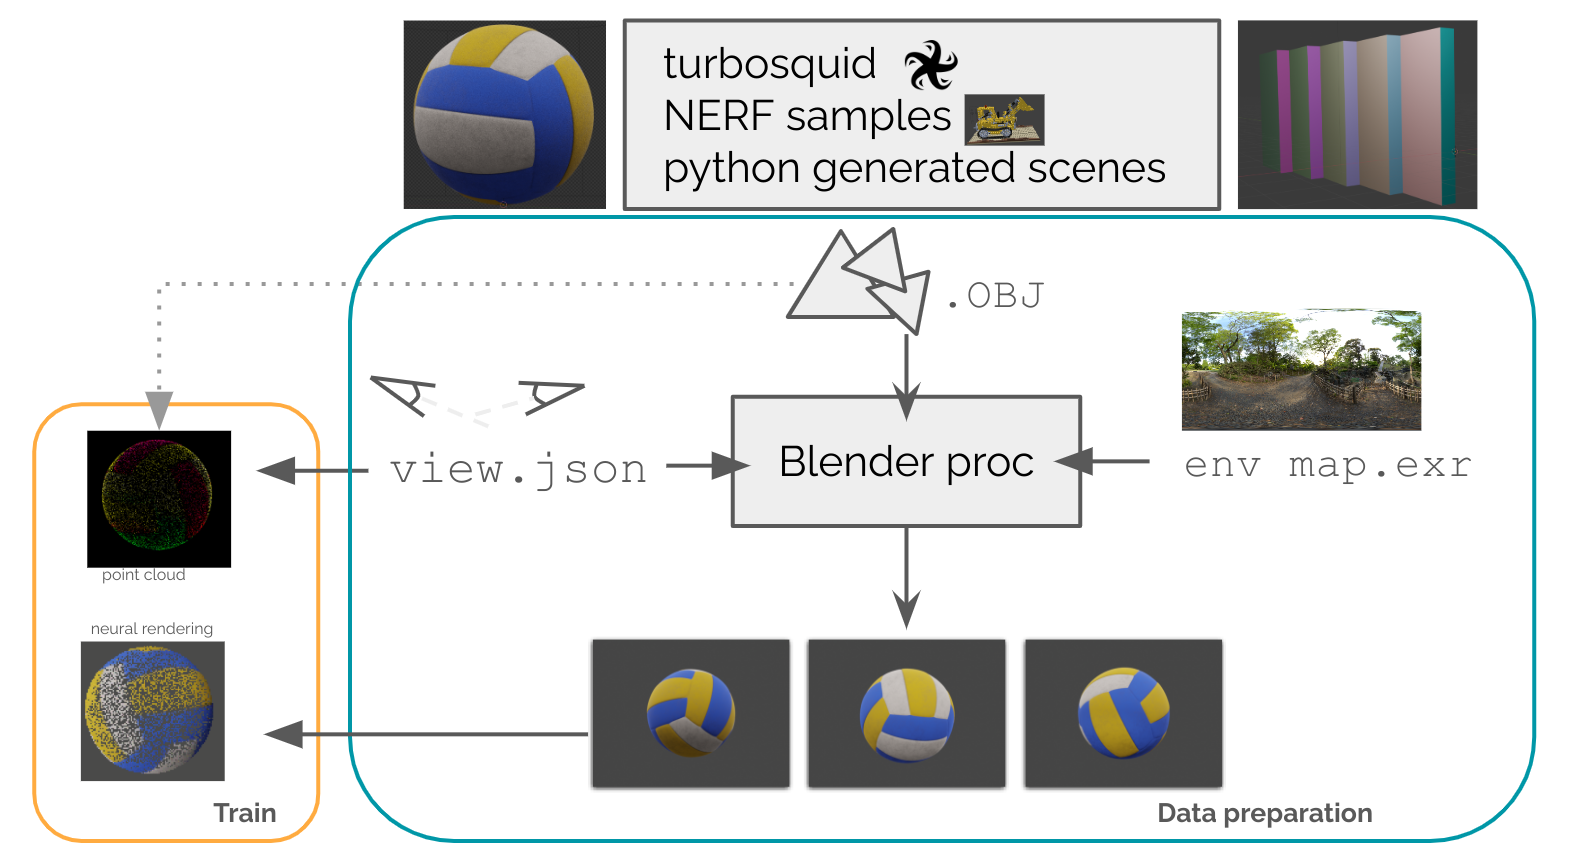
\includegraphics[width=0.5\textwidth]{figures/data_prep_and_training.png}
    \caption{Workflow: \href{https://github.com/balthazarneveu/per-pixel-point-rendering/blob/main/studies/photorealistic\_rendering.py}{\texttt{photorealistic\_rendering.py}} allows preparing multiple camera poses saved as \texttt{.json} files in order to render photorealistic views of a \texttt{.blend} or mesh \texttt{.obj} files which come from internet resources (TurboSquid/NERF sample dataset) or test scenes generated in python.
    The .obj and view .json files tie together the BlenderProc rendering and my Pytorch point rendering implementation: The point cloud is sampled from the mesh and the camera poses are known. A neural network is trained using \href{https://github.com/balthazarneveu/per-pixel-point-rendering/blob/main/scripts/optimize\_point\_based\_neural\_renderer.py}{\texttt{optimize\_point\_based\_neural\_renderer.py}} to predict colors of the points by trying to match the multiple photorealistic renderings. CNN weights, pointcloud, normals and pseudo-colors are all saved along in a \texttt{.pt} file which later allows performing live novel view synthesis \href{https://github.com/balthazarneveu/per-pixel-point-rendering/blob/main/scripts/novel\_views\_interactive.py}{\texttt{novel\_views\_interactive.py}} based on my own library \href{https://github.com/balthazarneveu/interactive\_pipe}{interactive\_pipe}}.
    \label{fig:data_and_train}
\end{figure*}



% \begin{table*}[htpb]
%     \begin{tabular}{|l|l|l|l|l|l|}
%     \hline
%     Number of points & PSNR   & Mode     & Conv size & Pseudo color dimension & Multi-scale supervision \\ \hline
%     100k             & 16.7dB & Bypass   & 1x1               & 3                      & Yes                     \\ \hline
%     100k             & 21.2dB & Conv 5x5 & 5x5               & 3                      & Yes                     \\ \hline
%     100k             & 26.3dB & Vanilla  & 5x5               & 8                      & No                      \\ \hline
%     100k             & \textbf{29dB}   & Vanilla  & 5x5               & 8                      & Yes                     \\ \hline
%     400k             & 23dB   & Bypass   & 1x1               & 3                      & No                      \\ \hline
%     800k             & 25db   & Bypass   & 1x1               & 3                      & No                      \\ \hline
% \end{tabular}
% \caption{Quantitative performances (PSNR on validation set) of various training configurations on the \texttt{Old chair} scene.}
% \label{tab:results}
% \end{table*}


% \begin{figure}[H]
%     \centering
%     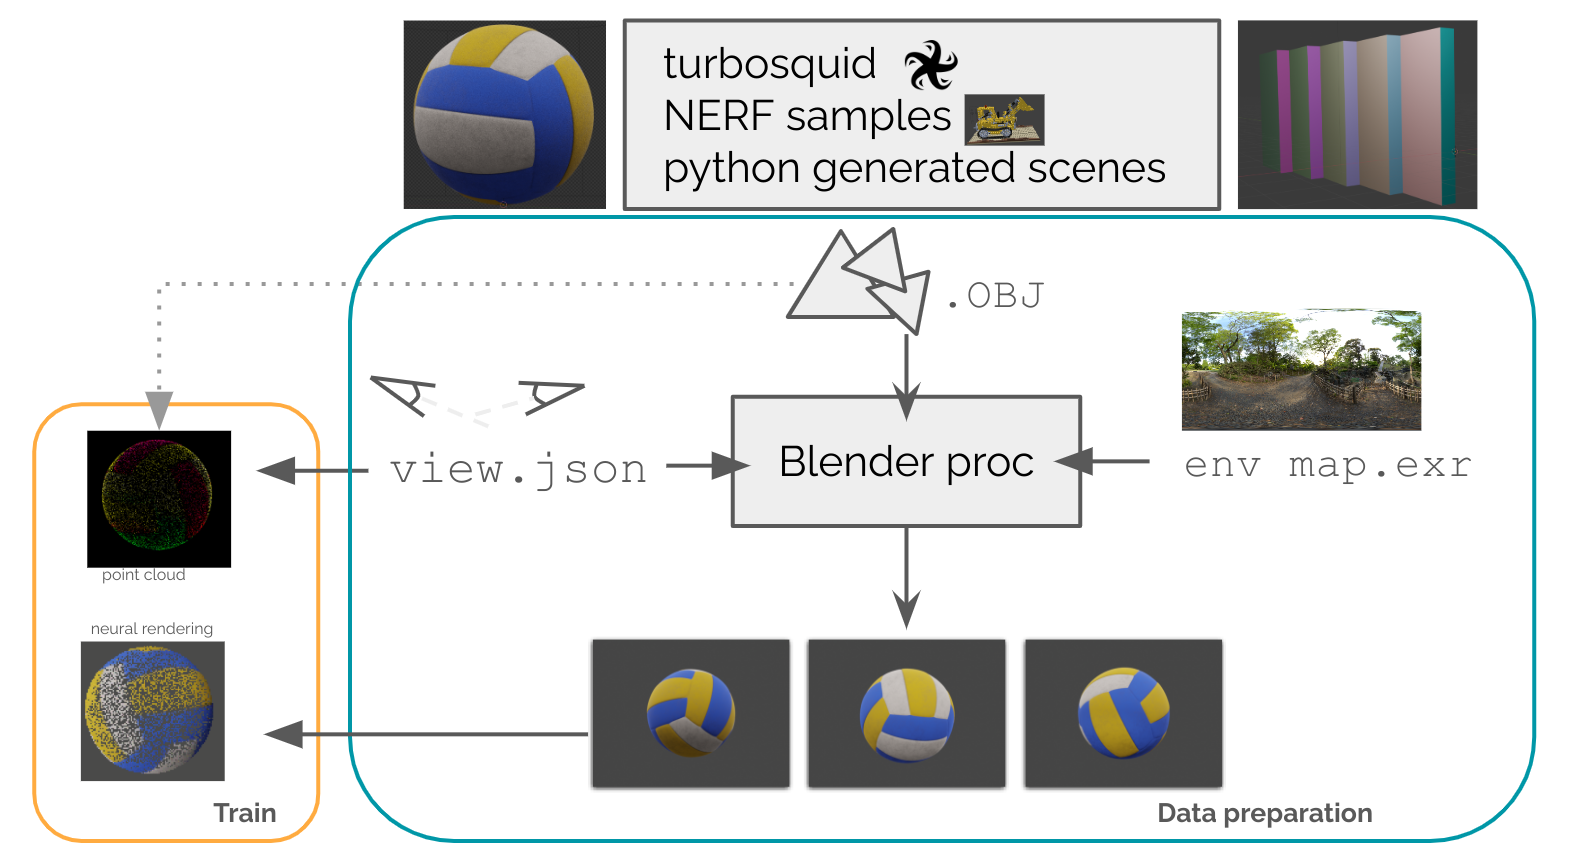
\includegraphics[width=0.45\textwidth]{figures/data_prep_and_training.png}
%     \caption{Workflow: \href{https://github.com/balthazarneveu/per-pixel-point-rendering/blob/main/studies/photorealistic\_rendering.py}{\texttt{photorealistic\_rendering.py}} allows preparing camera multiviews positions saved as \texttt{.json} files in order to render photorealistic views of a \texttt{.blend} or  \texttt{.obj} files which come from internet resources or test scenes generated in python.
%     The .obj and view .json files tie together the BlenderProc rendering and my Pytorch point rendering implementation: The point cloud is sampled from the mesh and the camera poses are known. A neural network is trained using \href{https://github.com/balthazarneveu/per-pixel-point-rendering/blob/main/scripts/optimize\_point\_based\_neural\_renderer.py}{\texttt{optimize\_point\_based\_neural\_renderer.py}} to predict colors of the points by trying to match the multiple photorealistic renderings. CNN weights, pointcloud, normals and pseudo-colors are all saved along in a \texttt{.pt} file which later allows performing live novel view synthesis \href{https://github.com/balthazarneveu/per-pixel-point-rendering/blob/main/scripts/novel\_views\_interactive.py}{\texttt{novel\_views\_interactive.py}} based on the self developped \href{https://github.com/balthazarneveu/interactive\_pipe}{interactive\_pipe} library}.
%     \label{fig:data_and_train}
% \end{figure}


% \begin{figure}[htpb]
%     \centering
%     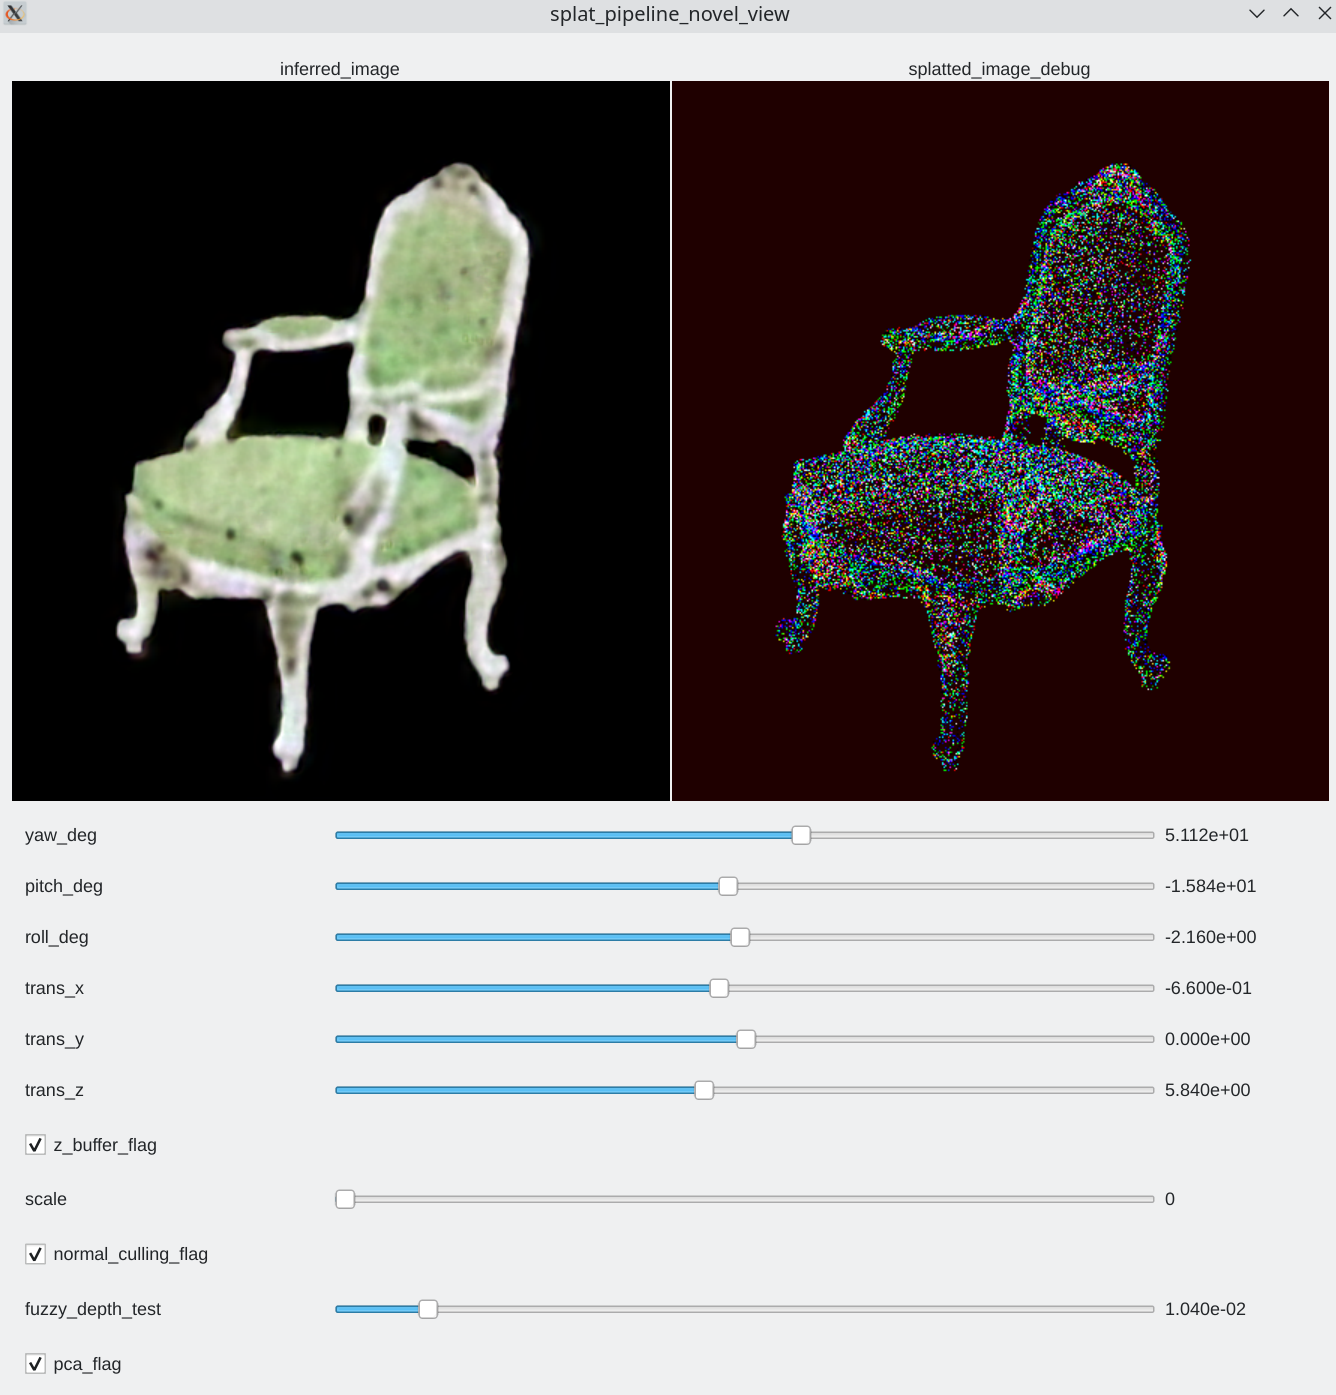
\includegraphics[width=0.45\textwidth]{figures/inference_live.png}
%     \caption{Live inference, the user can move the camera around the scene and see the novel view rendered in real time. On the right side we visualize the projected pseudo colored point cloud of dimension 8 using a Principal Component Analyzis.}
%     \label{fig:live_inference}
% \end{figure}


\end{document}
